\documentclass[11pt,a4paper,oneside]{report}

% ==============================================================================
% PACCHETTI FONDAMENTALI
% ==============================================================================
\usepackage[utf8]{inputenc}
\usepackage[T1]{fontenc}
\usepackage[italian]{babel}
\usepackage{lmodern}
\usepackage{microtype}
\usepackage{graphicx}
\usepackage{caption}
\captionsetup{font={small,sf}, labelfont=bf}
\usepackage[top=2.5cm, bottom=2.5cm, left=2.5cm, right=2.5cm]{geometry}

% Matematica avanzata
\usepackage{amsmath,amssymb,amsthm,mathtools,bm}
\usepackage{mathrsfs}

% Tabelle e impaginazione
\usepackage{booktabs}
\usepackage{tabularx}
\usepackage{array}
\usepackage{multirow}
\usepackage{enumitem}
\usepackage{fancyhdr}
\usepackage{titlesec}

% Colori e Box grafici
\usepackage{xcolor}
\usepackage[most]{tcolorbox}

% Grafici TikZ e PGFPlots
\usepackage{tikz}
\usepackage{pgfplots}
\pgfplotsset{compat=1.18}
\usetikzlibrary{arrows.meta,calc,patterns,babel,decorations.pathreplacing}

% Configurazione per sistemi di equazioni con parentesi graffe ampie e proporzionate
\renewcommand{\arraystretch}{1.4}
\newenvironment{sistema}[1][1.5]{%
    \renewcommand{\arraystretch}{#1}%
    \left\{%
    \begin{array}{@{}l@{}}%
}{%
    \end{array}%
    \right.%
}

% Collegamenti ipertestuali
\usepackage[colorlinks=true,
            linkcolor=blue!80!black,
            citecolor=teal!80!black,
            urlcolor=cyan!80!black,
            bookmarksdepth=3]{hyperref}

% ==============================================================================
% DEFINIZIONE DELLA PALETTE COLORI ISTITUZIONALE
% ==============================================================================
\definecolor{primaryBlue}{RGB}{24, 76, 120}
\definecolor{accentTeal}{RGB}{18, 120, 115}
\definecolor{lightGray}{RGB}{245, 247, 250}
\definecolor{borderGray}{RGB}{209, 213, 219}
\definecolor{slateBorder}{RGB}{203, 213, 225}
\definecolor{alertRed}{RGB}{185, 28, 28}
\definecolor{accentRed}{RGB}{220, 38, 38}
\definecolor{warningAmber}{RGB}{217, 119, 6}
\definecolor{accentAmber}{RGB}{217, 119, 6}
\definecolor{examplePurple}{RGB}{109, 40, 217}
\definecolor{methodSlate}{RGB}{51, 65, 85}
\definecolor{formulaGreen}{RGB}{16, 122, 80}
\definecolor{accentGreen}{RGB}{22, 163, 74}

% ==============================================================================
% CONFIGURAZIONE AMBIENTI GRAFICI TCOLORBOX
% ==============================================================================

% 1. Definizione
\newtcolorbox[auto counter, number within=chapter]{definizione}[1][]{
    enhanced,
    colback=primaryBlue!5!white,
    colframe=primaryBlue,
    coltitle=white,
    fonttitle=\bfseries\sffamily,
    title=Definizione~\thetcbcounter\ifstrempty{#1}{}{: #1},
    sharp corners=northwest,
    arc=3mm,
    boxrule=1.2pt,
    top=3mm, bottom=3mm, left=4mm, right=4mm,
    before skip=4mm, after skip=4mm
}

% 2. Teorema
\newtcolorbox[auto counter, number within=chapter]{teorema}[1][]{
    enhanced,
    colback=accentTeal!6!white,
    colframe=accentTeal,
    coltitle=white,
    fonttitle=\bfseries\sffamily,
    title=Teorema~\thetcbcounter\ifstrempty{#1}{}{: #1},
    sharp corners=northwest,
    arc=3mm,
    boxrule=1.2pt,
    top=3mm, bottom=3mm, left=4mm, right=4mm,
    before skip=4mm, after skip=4mm
}

% 2b. Corollario
\newtcolorbox[auto counter, number within=chapter]{corollario}[1][]{
    enhanced,
    colback=accentTeal!4!white,
    colframe=accentTeal!80!black,
    coltitle=white,
    fonttitle=\bfseries\sffamily,
    title=Corollario~\thetcbcounter\ifstrempty{#1}{}{: #1},
    sharp corners=northwest,
    arc=3mm,
    boxrule=1pt,
    top=3mm, bottom=3mm, left=4mm, right=4mm,
    before skip=4mm, after skip=4mm
}

% 3. Dimostrazione
\newtcolorbox{dimostrazione}[1][Dimostrazione]{
    enhanced,
    blanker,
    breakable,
    left=4mm,
    before skip=3mm, after skip=4mm,
    borderline west={2.5pt}{0pt}{accentTeal!70!black},
    fontupper=\small,
    title={\bfseries\sffamily\color{accentTeal!80!black} #1.},
    attach title to upper={\par\vspace{1.5mm}}
}

% 4. Esercizio Svolto
\newtcolorbox[auto counter, number within=chapter]{esercizio}[1][]{
    enhanced,
    colback=examplePurple!5!white,
    colframe=examplePurple!90!black,
    coltitle=white,
    fonttitle=\bfseries\sffamily,
    title=Esercizio Svolto~\thetcbcounter\ifstrempty{#1}{}{: #1},
    arc=2mm,
    boxrule=1pt,
    top=3mm, bottom=3mm, left=4mm, right=4mm,
    before skip=4mm, after skip=4mm
}

% 5. Esempio
\newtcolorbox[auto counter, number within=chapter]{esempio}[1][]{
    enhanced,
    colback=warningAmber!6!white,
    colframe=warningAmber!90!black,
    coltitle=white,
    fonttitle=\bfseries\sffamily,
    title=Esempio Guida~\thetcbcounter\ifstrempty{#1}{}{: #1},
    arc=2mm,
    boxrule=1pt,
    top=3mm, bottom=3mm, left=4mm, right=4mm,
    before skip=4mm, after skip=4mm
}

% 6. Attenzione / Errore Didattico Frequente
\newtcolorbox{attenzione}[1][Attenzione: Errore Ricorrente]{
    enhanced,
    colback=alertRed!6!white,
    colframe=alertRed,
    coltitle=white,
    fonttitle=\bfseries\sffamily,
    title=\textbf{#1},
    arc=2mm,
    boxrule=1.2pt,
    top=3mm, bottom=3mm, left=4mm, right=4mm,
    before skip=4mm, after skip=4mm
}

% 7. Metodo Operativo / Schema di Calcolo
\newtcolorbox{metodo}[1][Schema Metodologico]{
    enhanced,
    colback=methodSlate!5!white,
    colframe=methodSlate,
    coltitle=white,
    fonttitle=\bfseries\sffamily,
    title=#1,
    arc=2mm,
    boxrule=1.2pt,
    top=3mm, bottom=3mm, left=4mm, right=4mm,
    before skip=4mm, after skip=4mm
}

% ==============================================================================
% CONFIGURAZIONE HEADER E FOOTER
% ==============================================================================
\pagestyle{fancy}
\fancyhf{}
\fancyhead[L]{\small\sffamily\color{gray}Quaderno del Prof -- Classe 4F}
\fancyhead[R]{\small\sffamily\color{gray}Esponenziali, Logaritmi e Goniometria}
\fancyfoot[C]{\small\sffamily\thepage}
\renewcommand{\headrulewidth}{0.4pt}
\renewcommand{\footrulewidth}{0pt}

% Titoli delle sezioni con font sans-serif elegante
\titleformat{\chapter}[display]
  {\normalfont\sffamily\huge\bfseries\color{primaryBlue}}
  {\chaptertitlename\ \thechapter}{15pt}{\Huge}
\titleformat{\section}
  {\normalfont\sffamily\Large\bfseries\color{primaryBlue}}
  {\thesection}{1em}{}
\titleformat{\subsection}
  {\normalfont\sffamily\large\bfseries\color{accentTeal}}
  {\thesubsection}{1em}{}

% ==============================================================================
% INIZIO DOCUMENTO
% ==============================================================================
\begin{document}

% ------------------------------------------------------------------------------
% FRONTESPIZIO
% ------------------------------------------------------------------------------
\begin{titlepage}
    \centering
    \vspace*{2.0cm}
    
    {\fontsize{34}{42}\selectfont\sffamily\bfseries\color{primaryBlue} Quaderno del Prof}\\[0.6cm]
    {\Large\sffamily\bfseries\color{accentTeal} Matematica e Fisica}\\[0.3cm]
    {\large\sffamily\color{methodSlate} Teoria Completa, Dimostrazioni Passo-Passo ed Esercizi Risolti}\\[1.5cm]
    
    \rule{0.85\linewidth}{1.5pt}\\[1.8cm]
    
    {\huge\sffamily\bfseries ESPONENZIALI, LOGARITMI\\ E INTRODUZIONE ALLA GONIOMETRIA}\\[1.8cm]
    
    \rule{0.85\linewidth}{1.5pt}\\[2.5cm]
    
    {\Large\sffamily
    \textbf{Liceo Scientifico Statale «Leonardo da Vinci» -- Maglie}\\[0.3cm]
    Classe: \textbf{4F MAT}\\[0.2cm]
    Materia: \textbf{Matematica e Fisica}\\[0.4cm]
    \large\color{primaryBlue}\textbf{Edizione Completa Monografica -- 31 Pagine Autentiche di Appunti}
    }
    
    \vfill
\end{titlepage}

% ------------------------------------------------------------------------------
% INDICE GENERALE
% ------------------------------------------------------------------------------
\tableofcontents
\newpage

% ==============================================================================
% CAPITOLO 1: FUNZIONE ESPONENZIALE E COSTANTE DI NEPERO
% ==============================================================================
\chapter{La Funzione Esponenziale e la Costante di Nepero}

\section{La Genesi del Numero $e$: Il Problema di Jacob Bernoulli}
Il numero trascendente $e \approx 2{,}718281828459\dots$, noto storicamente come \emph{costante di Eulero} o \emph{numero di Nepero}, trae la propria origine formale dall'analisi finanziaria della capitalizzazione composta intrapresa dal matematico svizzero Jacob Bernoulli nel 1683.

Consideriamo un capitale iniziale $C$ investito a un tasso nominale di rendimento annuo pari al $100\%$ ($r = 1$). Se l'interesse viene riconosciuto e liquidato esclusivamente alla fine dell'anno (capitalizzazione semplice annuale), il montante finale $M$ generato è:
\begin{equation}
    M = C + C \cdot 1 = C(1 + 1) = 2C
\end{equation}
Qualora il medesimo rendimento annuale venga frazionato in due semestri, a ciascuna scadenza semestrale corrisponderà un tasso parziale pari a $\frac{r}{2} = 50\% = 0{,}5$. Al termine del primo semestre il capitale accumulato diventa:
\begin{equation}
    M_{1/2} = C + C \cdot 0{,}5 = C(1 + 0{,}5) = 1{,}5 \, C
\end{equation}
Nel secondo semestre, l'interesse non matura solo sul capitale primitivo $C$, bensì sull'intero montante $M_{1/2}$ maturato (regime di interesse composto):
\begin{equation}
    M_1 = M_{1/2} + M_{1/2} \cdot 0{,}5 = M_{1/2}(1 + 0{,}5) = C(1 + 0{,}5)(1 + 0{,}5) = C\left(1 + \frac{1}{2}\right)^2 = 2{,}25 \, C
\end{equation}
Generalizzando il procedimento a una suddivisione dell'anno in $n$ sotto-periodi omogenei (quadrimestri con $n=3$, trimestri con $n=4$, mesi con $n=12$, giorni con $n=365$), il tasso per ciascun periodo è $\frac{1}{n}$ e il montante finale dopo un anno è governato dalla legge:
\begin{equation}
    M_n = C\left(1 + \frac{1}{n}\right)^n
\end{equation}

\begin{table}[htbp]
\centering
\small
\caption{Convergenza del montante $M_n$ per $C = 1000\text{ euro}$ al crescere delle frazioni temporali $n$.}
\label{tab:bernoulli}
\begin{tabularx}{\textwidth}{l c >{\centering\arraybackslash}X r}
\toprule
\textbf{Frequenza} & \textbf{Periodi ($n$)} & \textbf{Formula analitica} & \textbf{Montante finale (EUR)} \\
\midrule
Annuale & $n = 1$ & $1000 \cdot (1 + 1)^1$ & $2000{,}00$ \\
Semestrale & $n = 2$ & $1000 \cdot (1 + 0{,}5)^2$ & $2250{,}00$ \\
Quadrimestrale & $n = 3$ & $1000 \cdot (1 + 1/3)^3$ & $2370{,}37$ \\
Trimestrale & $n = 4$ & $1000 \cdot (1 + 0{,}25)^4$ & $2441{,}41$ \\
Mensile & $n = 12$ & $1000 \cdot (1 + 1/12)^{12}$ & $2613{,}04$ \\
Giornaliero & $n = 365$ & $1000 \cdot (1 + 1/365)^{365}$ & $2714{,}57$ \\
Orario & $n = 8760$ & $1000 \cdot (1 + 1/8760)^{8760}$ & $2718{,}13$ \\
Al secondo & $n = 31\,536\,000$ & $1000 \cdot (1 + 1/n)^n$ & $2718{,}28$ \\
\textbf{Continua (istante per istante)} & \textbf{Stabilizzazione} & $\mathbf{1000 \cdot e}$ & $\mathbf{2718{,}2818\dots}$ \\
\bottomrule
\end{tabularx}
\end{table}

\begin{figure}[htbp]
\centering
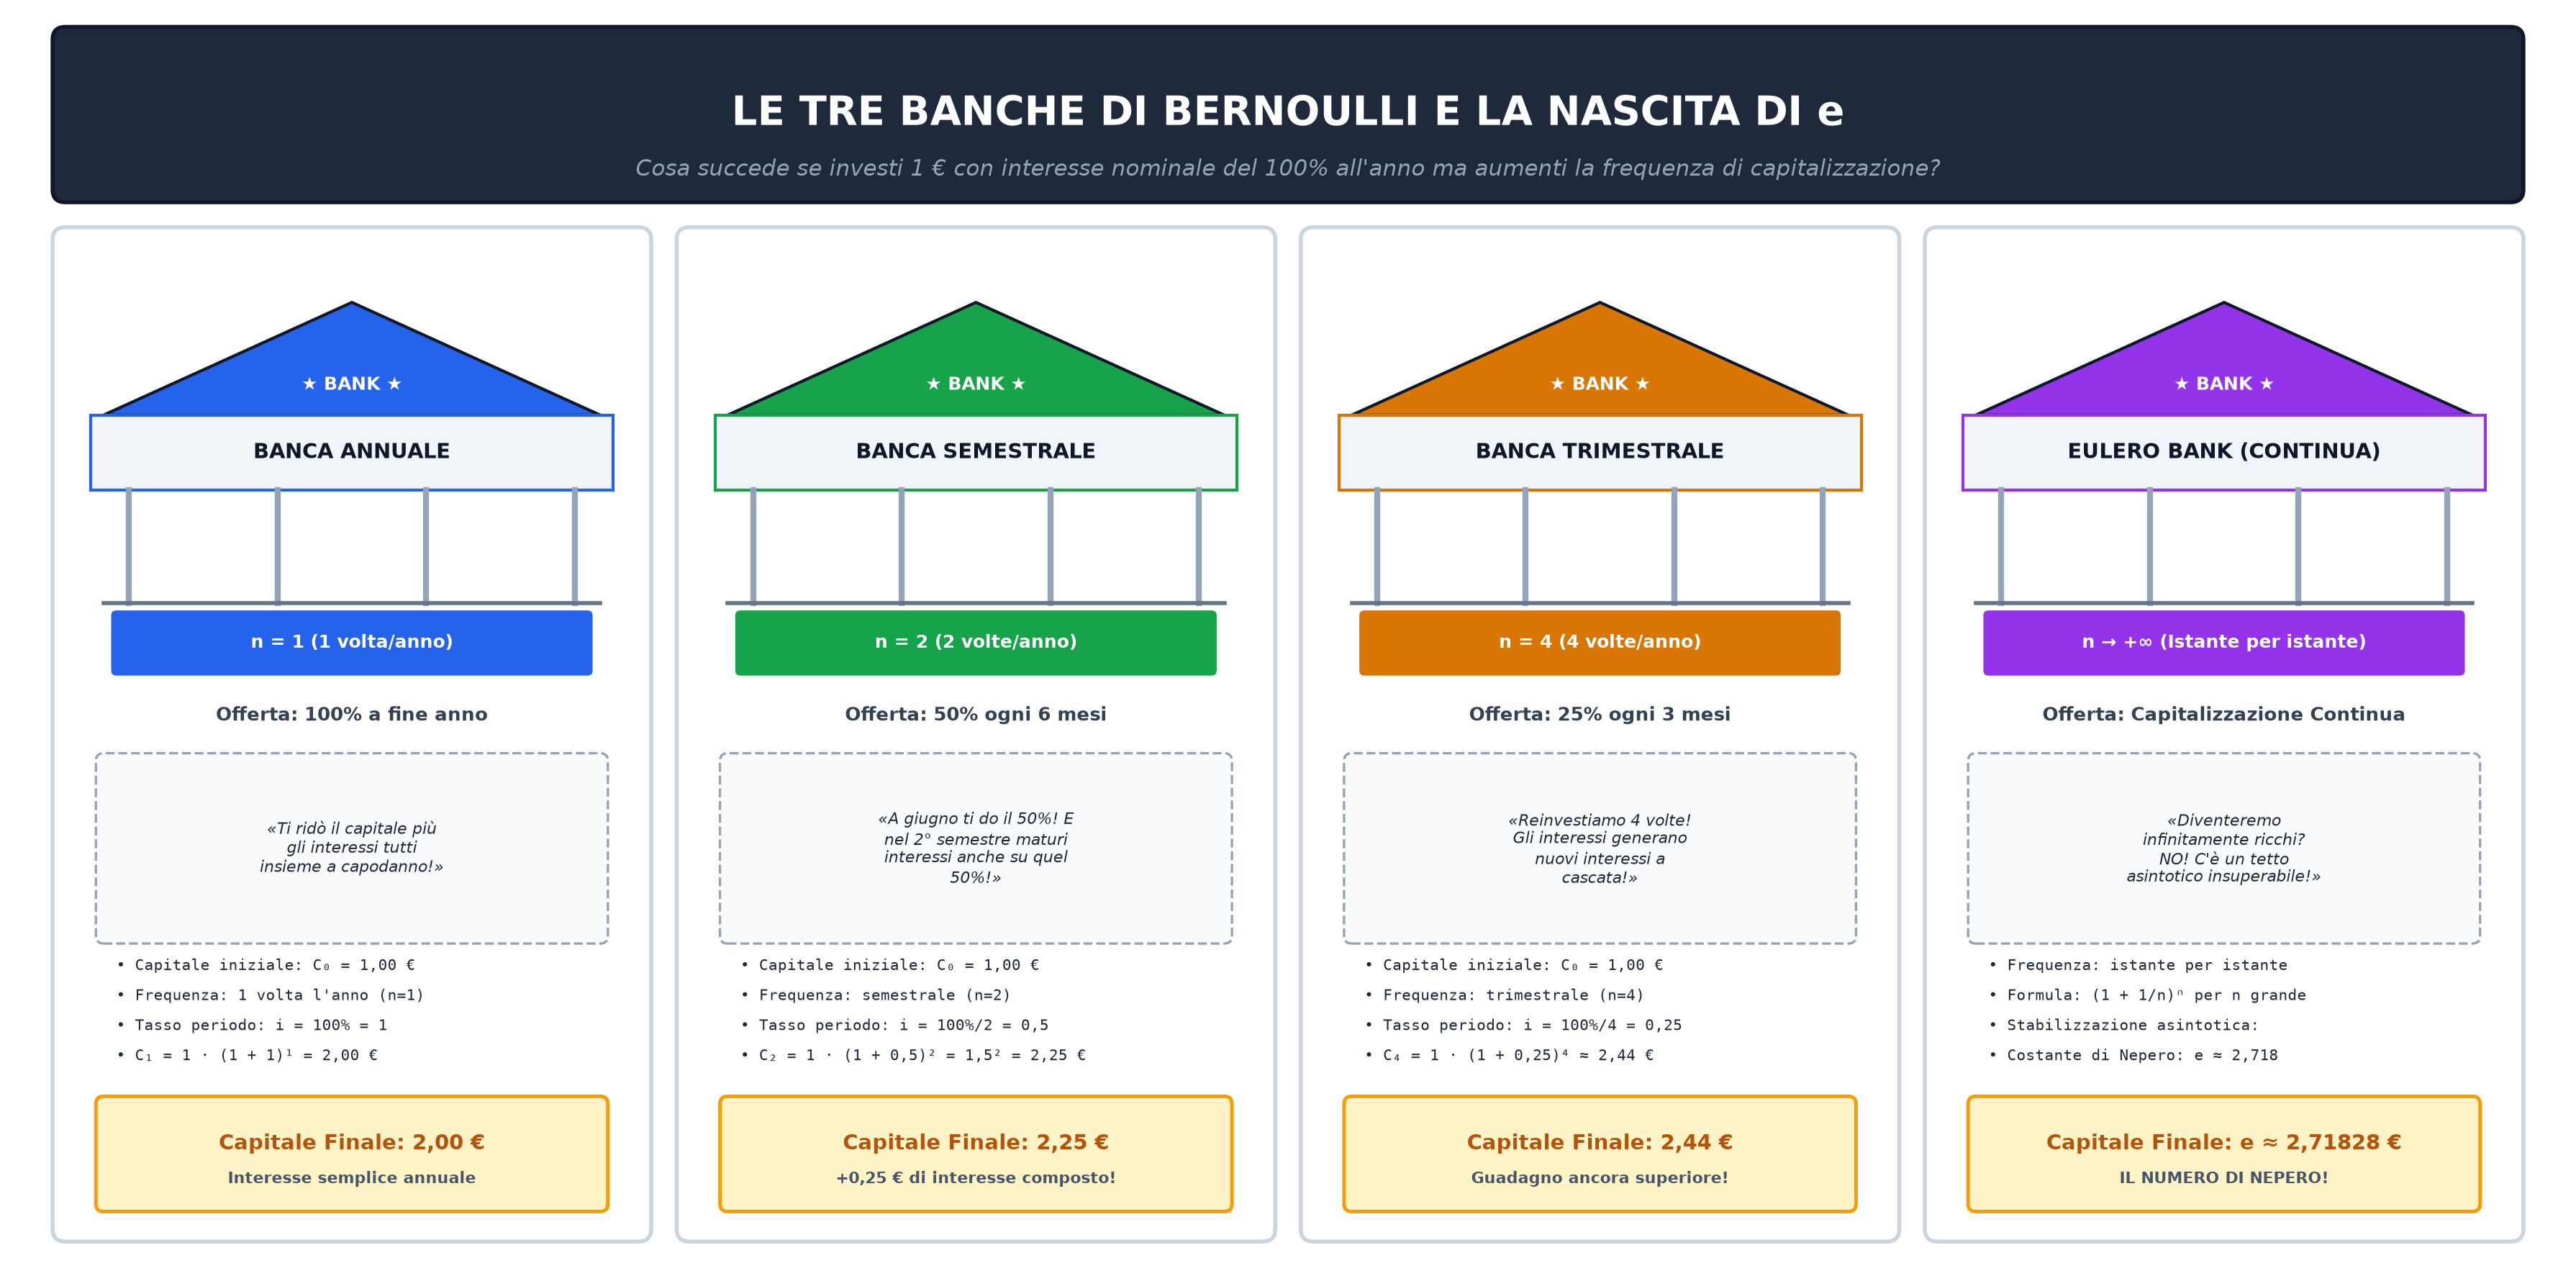
\includegraphics[width=0.96\textwidth]{immagini/bernoulli_banche_fumetto.png}
\caption{Striscia e infografica didattica: Il paradosso economico di Jacob Bernoulli e il confronto tra le banche (annuale 100\%, semestrale 50\%, trimestrale 25\%) fino alla soglia asintotica insuperabile del numero di Nepero $e \approx 2{,}71828\dots\text{ EUR}$.}
\label{fig:banche_bernoulli}
\end{figure}

\begin{teorema}[La Costante di Nepero $e$]
All'aumentare indefinito del numero $n$ di suddivisioni temporali nella capitalizzazione composta, i valori della successione:
\begin{equation}
    a_n = \left(1 + \frac{1}{n}\right)^n, \quad n \in \mathbb{N}^+
\end{equation}
crescono progressivamente mantenendosi sempre inferiori a $3$. La successione si stabilizza così verso un valore numerico costante e insuperabile, indicato universalmente con la lettera $e$:
\begin{equation}
    e \approx 2{,}718281828459\dots
\end{equation}
\end{teorema}

\begin{dimostrazione}[\bfseries Dimostrazione Analitica (Approfondimento Facoltativo)]
Utilizzando lo sviluppo del binomio di Newton:
\begin{align*}
    a_n &= \left(1 + \frac{1}{n}\right)^n = \sum_{k=0}^n \binom{n}{k} \frac{1}{n^k} \\
    &= 1 + n \cdot \frac{1}{n} + \frac{n(n-1)}{2!} \frac{1}{n^2} + \frac{n(n-1)(n-2)}{3!} \frac{1}{n^3} + \dots + \frac{n(n-1)\dots 1}{n!} \frac{1}{n^n} \\
    &= 1 + 1 + \frac{1}{2!}\left(1 - \frac{1}{n}\right) + \frac{1}{3!}\left(1 - \frac{1}{n}\right)\left(1 - \frac{2}{n}\right) + \dots + \frac{1}{n!}\left(1 - \frac{1}{n}\right)\dots\left(1 - \frac{n-1}{n}\right)
\end{align*}
Ciascun addendo è positivo. All'aumentare di $n$ a $n+1$, compaiono sia un termine aggiuntivo positivo, sia fattori moltiplicativi $\left(1 - \frac{k}{n}\right) < \left(1 - \frac{k}{n+1}\right)$ più grandi. Dunque $a_n < a_{n+1}$ (stretta crescenza).

Inoltre, poiché $\left(1 - \frac{k}{n}\right) < 1$ e per $k \ge 2$ si ha $k! \ge 2^{k-1}$:
\begin{equation}
    a_n < 1 + 1 + \frac{1}{2!} + \frac{1}{3!} + \dots + \frac{1}{n!} < 1 + 1 + \frac{1}{2} + \frac{1}{4} + \dots + \frac{1}{2^{n-1}} = 1 + \frac{1 - (1/2)^n}{1 - 1/2} < 1 + 2 = 3
\end{equation}
Essendo monotona crescente e limitata superiormente da 3, i valori della successione si stabilizzano e convergono a un valore finito compreso tra $2$ e $3$, identificato con la costante $e$.
\end{dimostrazione}

\section{Algebra delle Potenze ad Esponente Reale}
Prima di analizzare la funzione esponenziale reale, richiamiamo le proprietà fondamentali delle potenze. Siano $a, b \in \mathbb{R}^+$ ed $x, y \in \mathbb{R}$:
\begin{enumerate}[label=\textbf{\arabic*.}]
    \item $a^x \cdot a^y = a^{x+y}$
    \item $\dfrac{a^x}{a^y} = a^{x-y}$
    \item $(a^x)^y = a^{x \cdot y}$
    \item $(a \cdot b)^x = a^x \cdot b^x$
    \item $\left(\dfrac{a}{b}\right)^x = \dfrac{a^x}{b^x}$
    \item $a^{-x} = \dfrac{1}{a^x}$
    \item $a^{m/n} = \sqrt[n]{a^m} \quad (m \in \mathbb{Z}, n \in \mathbb{N}^+)$
\end{enumerate}

\section{Definizione e Proprietà della Funzione Esponenziale}

\begin{definizione}[Funzione Esponenziale]
Si definisce \emph{funzione esponenziale elementare di base $a$} l'applicazione:
\begin{equation}
    f \colon \mathbb{R} \to \mathbb{R}^+, \quad f(x) = a^x
\end{equation}
con il vincolo fondamentale di ammissibilità della base:
\begin{equation}
    a > 0 \quad \text{e} \quad a \neq 1
\end{equation}
\end{definizione}

\begin{attenzione}[Perché la base $a$ deve soddisfare $a > 0$ ed $a \neq 1$?]
\begin{itemize}
    \item Se $a < 0$: l'espressione $a^x$ perde di significato reale per infiniti esponenti frazionari. Ad esempio, per $a = -4$ e $x = 1/2$, si avrebbe $(-4)^{1/2} = \sqrt{-4} \notin \mathbb{R}$. La funzione non sarebbe definibile in un intervallo continuo.
    \item Se $a = 0$: si avrebbe $0^x = 0$ per ogni $x > 0$, mentre per $x \le 0$ l'espressione risulterebbe indeterminata ($0^0$) o priva di significato ($0^{-1} = 1/0$).
    \item Se $a = 1$: l'espressione $1^x = 1$ degenera nella retta orizzontale costante $y = 1$, perdendo la caratteristica di biiettività essenziale per definire il logaritmo.
\end{itemize}
\end{attenzione}

\subsection{Caratteristiche Analitiche e Asintoti}
\begin{itemize}
    \item \textbf{Dominio:} $\mathcal{D} = \mathbb{R} = (-\infty, +\infty)$.
    \item \textbf{Codominio (Insieme Immagine):} $\mathrm{Im}(f) = \mathbb{R}^+ = (0, +\infty)$. L'esponenziale reale è sempre strettamente positiva:
    \begin{equation}
        a^x > 0 \quad \forall x \in \mathbb{R}
    \end{equation}
    \item \textbf{Punto fisso fondamentale:} Per ogni $a$, si ha $a^0 = 1$, dunque il grafico interseca l'asse delle ordinate nel punto $P(0, 1)$. Inoltre passa per $(1, a)$.
    \item \textbf{Biforcazione della monotonia:}
    \begin{itemize}
        \item Se $\mathbf{a > 1}$: la funzione è \textbf{strettamente crescente}:
        \begin{equation}
            x_1 < x_2 \iff a^{x_1} < a^{x_2}
        \end{equation}
        Comportamento asintotico e andamento globale:
        \begin{itemize}
            \item Per valori di $x$ negativi di modulo sempre più grande ($x \to -\infty$), i valori di $a^x$ si avvicinano sempre più alla retta $y = 0$ senza mai toccarla (\textbf{asintoto orizzontale sinistro}: $y = 0$).
            \item Per valori di $x$ positivi via via crescenti ($x \to +\infty$), i valori di $a^x$ crescono indefinitamente verso l'alto ($y \to +\infty$).
        \end{itemize}
        \item Se $\mathbf{0 < a < 1}$: la funzione è \textbf{strettamente decrescente}:
        \begin{equation}
            x_1 < x_2 \iff a^{x_1} > a^{x_2}
        \end{equation}
        Comportamento asintotico e andamento globale:
        \begin{itemize}
            \item Per valori di $x$ negativi di modulo sempre più grande ($x \to -\infty$), i valori della funzione crescono indefinitamente verso l'alto ($y \to +\infty$).
            \item All'aumentare indefinito di $x$ verso valori positivi ($x \to +\infty$), la curva si avvicina sempre più alla retta $y = 0$ senza mai toccarla (\textbf{asintoto orizzontale destro}: $y = 0$).
        \end{itemize}
    \end{itemize}
    \item \textbf{Simmetria speculare tra basi reciproche:} Poiché $\left(\frac{1}{a}\right)^x = a^{-x}$, la curva $y = \left(\frac{1}{a}\right)^x$ si ottiene da $y = a^x$ mediante una riflessione assiale rispetto all'asse delle ordinate $y$ ($x \mapsto -x$).
\end{itemize}

\section{Rappresentazione Grafica Comparativa}

\begin{figure}[htbp]
\centering
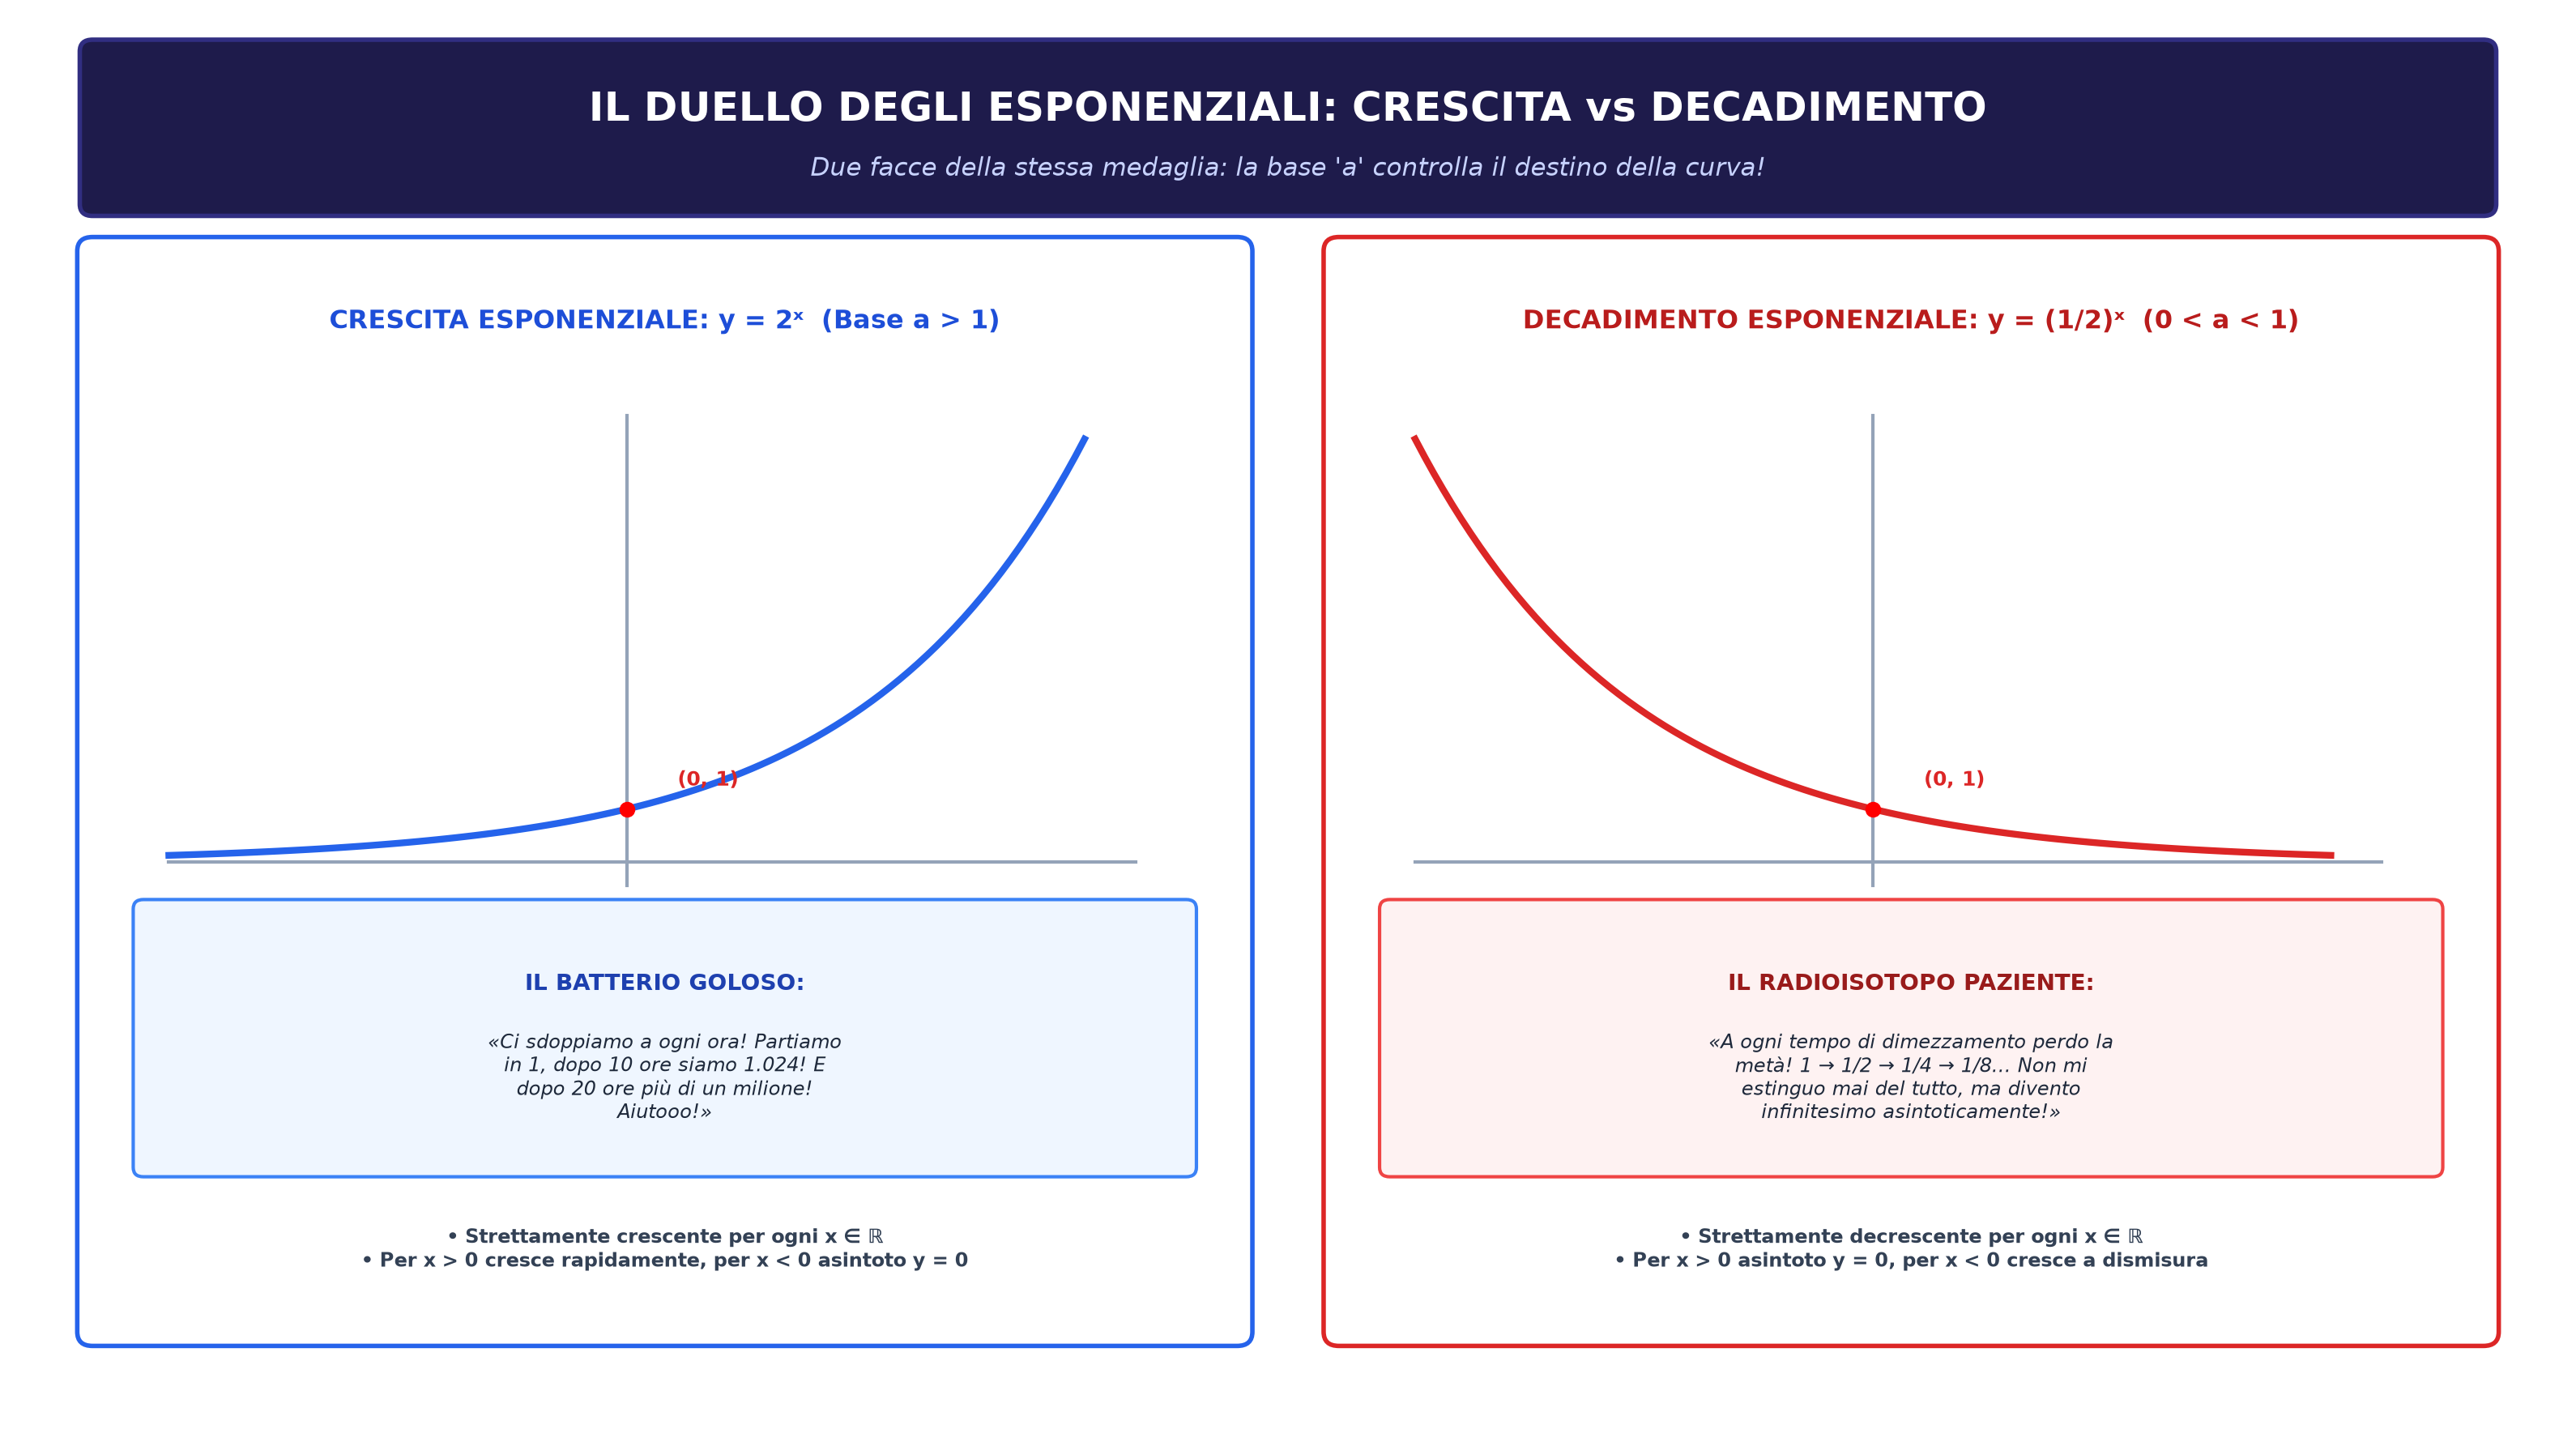
\includegraphics[width=0.92\textwidth]{immagini/duello_esponenziali.png}
\caption{Infografica comparativa: Il duello degli esponenziali. La base $a > 1$ governa la moltiplicazione esponenziale ($y = 2^x$), mentre $0 < a < 1$ governa il decadimento asintotico a tempo di dimezzamento ($y = (1/2)^x$).}
\label{fig:duello_esponenziali}
\end{figure}

\begin{figure}[htbp]
\centering
\begin{tikzpicture}
\begin{axis}[
    axis lines=middle,
    xlabel={$x$},
    ylabel={$y$},
    xmin=-3.5, xmax=3.5,
    ymin=-0.5, ymax=6.5,
    samples=120,
    grid=both,
    grid style={line width=.1pt, draw=gray!25},
    major grid style={line width=.25pt, draw=gray!40},
    axis line style={-{Latex[scale=1.2]}},
    ticklabel style={font=\footnotesize},
    xlabel style={at={(ticklabel* cs:1)},anchor=west},
    ylabel style={at={(ticklabel* cs:1)},anchor=south},
    width=12cm, height=7.5cm,
    legend pos=north west,
    legend cell align={left}
]
    % Curva a > 1: y = 2^x
    \addplot[primaryBlue, line width=1.6pt, domain=-3.5:2.6] {2^x};
    \addlegendentry{$y = 2^x \quad (a = 2 > 1, \text{ strett. crescente})$}
    
    % Curva 0 < a < 1: y = (1/2)^x
    \addplot[alertRed, line width=1.6pt, domain=-2.6:3.5] {(1/2)^x};
    \addlegendentry{$y = \left(\frac{1}{2}\right)^x = 2^{-x} \quad (0 < a < 1, \text{ strett. decrescente})$}
    
    % Asintoto orizzontale
    \draw[dashed, gray!80, line width=0.8pt] (-3.5,0) -- (3.5,0);
    
    % Punti notevoli
    \filldraw[black] (0,1) circle (2.2pt) node[anchor=south west, font=\footnotesize] {$(0,1)$};
    \filldraw[primaryBlue] (1,2) circle (2pt) node[anchor=south east, font=\footnotesize] {$(1,2)$};
    \filldraw[alertRed] (-1,2) circle (2pt) node[anchor=south west, font=\footnotesize] {$(-1,2)$};
    \filldraw[primaryBlue] (-1,0.5) circle (1.8pt) node[anchor=north east, font=\footnotesize] {$(-1, 0.5)$};
    \filldraw[alertRed] (1,0.5) circle (1.8pt) node[anchor=north west, font=\footnotesize] {$(1, 0.5)$};
\end{axis}
\end{tikzpicture}
\caption{Confronto cartesiano tra la curva esponenziale a base intera $y = 2^x$ e la corrispondente a base frazionaria reciproca $y = (1/2)^x$. Si noti il passaggio per il punto comune $(0,1)$ e la perfetta simmetria rispetto all'asse $y$.}
\label{fig:confronto_esponenziali}
\end{figure}

\newpage

% ==============================================================================
% CAPITOLO 2: EQUAZIONI E DISEQUAZIONI ESPONENZIALI
% ==============================================================================
\chapter{Equazioni e Disequazioni Esponenziali}

\section{Tipologie di Equazioni Esponenziali e Metodi Risolutivi}
Un'equazione si dice \emph{esponenziale} quando l'incognita $x$ compare nell'esponente di almeno una potenza.

\subsection{1. Equazione Elementare \texorpdfstring{$a^x = b$}{a\^{}x = b}}
Dalla definizione di funzione esponenziale e dalla positività di $a^x$:
\begin{itemize}
    \item Se $\mathbf{b \le 0}$: l'equazione $a^x = b$ è \textbf{impossibile} in $\mathbb{R}$ ($\mathcal{S} = \emptyset$). Esempio: $3^x = -2$ o $5^x = 0$ non ammettono soluzioni reali.
    \item Se $\mathbf{b > 0}$: per la stretta monotonia (e quindi biiettività) della funzione $f(x) = a^x$, esiste una e una sola soluzione reale:
    \begin{equation}
        a^x = b \iff x = \log_a b
    \end{equation}
\end{itemize}

\subsection{2. Metodo di Riduzione alla Stessa Base}
Qualora entrambi i membri dell'equazione possano essere riscritti come potenze della medesima base $a$:
\begin{equation}
    a^{f(x)} = a^{g(x)} \iff f(x) = g(x)
\end{equation}

\begin{esempio}[Riconduzione a base comune]
Risolvere l'equazione:
\begin{equation*}
    \left(\frac{2}{3}\right)^{x^2 - 3} = \left(\frac{9}{4}\right)^{x}
\end{equation*}
Osserviamo che la frazione $\frac{9}{4}$ è il quadrato del reciproco di $\frac{2}{3}$:
\begin{equation*}
    \frac{9}{4} = \left(\frac{3}{2}\right)^2 = \left(\frac{2}{3}\right)^{-2} \implies \left(\frac{9}{4}\right)^x = \left(\frac{2}{3}\right)^{-2x}
\end{equation*}
Uguagliando gli esponenti:
\begin{equation*}
    x^2 - 3 = -2x \iff x^2 + 2x - 3 = 0 \iff (x + 3)(x - 1) = 0
\end{equation*}
Le soluzioni sono $\mathcal{S} = \{-3, 1\}$.
\end{esempio}

\subsection{3. Metodo della Variabile Ausiliaria}
Quando l'equazione presenta potenze con esponenti multipli, si effettua una sostituzione del tipo:
\begin{equation}
    t = a^x \quad \text{con il vincolo vincolante } t > 0
\end{equation}

\begin{esercizio}[Equazione con variabile ausiliaria]
Risolvere l'equazione trascendente:
\begin{equation*}
    4^x - 3 \cdot 2^{x+1} + 8 = 0
\end{equation*}
\textbf{Svolgimento:}
Riscriviamo le potenze in base 2:
\begin{equation*}
    4^x = (2^2)^x = (2^x)^2, \qquad 2^{x+1} = 2^x \cdot 2^1 = 2 \cdot 2^x
\end{equation*}
L'equazione diviene:
\begin{equation*}
    (2^x)^2 - 6 \cdot (2^x) + 8 = 0
\end{equation*}
Poniamo la variabile ausiliaria $t = 2^x > 0$:
\begin{equation*}
    t^2 - 6t + 8 = 0 \iff (t - 2)(t - 4) = 0 \implies t_1 = 2, \quad t_2 = 4
\end{equation*}
Entrambi i valori sono strettamente positivi, dunque accettabili. Risostituendo $t = 2^x$:
\begin{align*}
    2^x &= 2 \implies x = 1 \\
    2^x &= 4 = 2^2 \implies x = 2
\end{align*}
L'insieme delle soluzioni è $\mathcal{S} = \{1, 2\}$.
\end{esercizio}

\section{Risoluzione Grafica di Equazioni Trascendenti Miste}
Quando compaiono simultaneamente funzioni esponenziali e funzioni algebriche (polinomi, razionali fratte, radici), non è in generale possibile isolare algebricamente l'incognita. Si adotta allora il \textbf{metodo grafico}, associando l'equazione all'intersezione di due curve note nel piano cartesiano.

\begin{esercizio}[Risoluzione grafica di $2^x = 1 - x^2$]
Determinare il numero e il valore (esatto o approssimato) delle radici reali dell'equazione:
\begin{equation*}
    2^x = 1 - x^2
\end{equation*}
\textbf{Svolgimento:}
Scomponiamo l'equazione nel sistema cartesiano di due curve elementari:
\begin{equation*}
    \begin{cases}
        y = 2^x & \text{(curva esponenziale crescente, } P(0,1) \text{ e asintoto orizzontale } y=0\text{)} \\[1.6ex]
        y = 1 - x^2 & \text{(parabola con vertice in } V(0,1)\text{, concavità verso il basso e zeri in } \pm 1\text{)}
    \end{cases}
\end{equation*}

\begin{center}
\begin{tikzpicture}
\begin{axis}[
    axis lines=middle,
    xlabel={$x$},
    ylabel={$y$},
    xmin=-2.2, xmax=2.2,
    ymin=-1.5, ymax=2.5,
    samples=100,
    grid=both,
    grid style={line width=.1pt, draw=gray!25},
    axis line style={-{Latex[scale=1.2]}},
    ticklabel style={font=\footnotesize},
    width=10.5cm, height=6.5cm
]
    \addplot[primaryBlue, line width=1.5pt, domain=-2.2:1.2] {2^x} node[pos=0.85, left, font=\footnotesize] {$y = 2^x$};
    \addplot[alertRed, line width=1.5pt, domain=-1.6:1.6] {1 - x^2} node[pos=0.15, right, font=\footnotesize] {$y = 1 - x^2$};
    
    % Punti di intersezione
    \filldraw[examplePurple] (0,1) circle (2.5pt) node[above right, font=\footnotesize] {$A(0,1)$ (soluzione esatta $x_1 = 0$)};
    \filldraw[examplePurple] (-0.71, 0.6) circle (2.5pt) node[below left, font=\footnotesize] {$B(-0.71, 0.60)$ ($x_2 \approx -0.71$)};
\end{axis}
\end{tikzpicture}
\par\vspace{1.5mm}
{\small\itshape Risoluzione grafica di $2^x = 1 - x^2$: le due curve si intersecano esattamente nel vertice $A(0,1)$ e nel punto $B(-0{,}71, 0{,}60)$.}
\end{center}

Dall'ispezione grafica:
\begin{enumerate}
    \item Per $x = 0$: $2^0 = 1$ e $1 - 0^2 = 1$. L'uguaglianza è verificata identicamente. Dunque \textbf{$x_1 = 0$} è una radice intera esatta.
    \item Per $x > 0$: per $x \in (0, 1)$ si ha $2^x > 1$, mentre $1 - x^2 < 1$. Per $x \ge 1$ la parabola è negativa ($1 - x^2 \le 0$) mentre l'esponenziale è strettamente maggiore di 2. Dunque non vi sono altre soluzioni per $x > 0$.
    \item Per $x < 0$: consideriamo la funzione ausiliaria continua $g(x) = 2^x + x^2 - 1$.
    \begin{align*}
        g(-1) &= 2^{-1} + (-1)^2 - 1 = \frac{1}{2} + 1 - 1 = \frac{1}{2} > 0 \\
        g(-0{,}5) &= 2^{-0{,}5} + (-0{,}5)^2 - 1 = \frac{1}{\sqrt{2}} + 0{,}25 - 1 \approx 0{,}707 - 0{,}75 = -0{,}043 < 0
    \end{align*}
    Per il \emph{Teorema di Esistenza degli Zeri}, esistendo una variazione di segno nell'intervallo continuo $[-1, -0{,}5]$, esiste una seconda radice reale $x_2 \in (-1, -0{,}5)$. Con il metodo delle tangenti di Newton o bisezione si trova $x_2 \approx -0{,}714$.
\end{enumerate}
\end{esercizio}

\section{Disequazioni Esponenziali}
La risoluzione delle disequazioni esponenziali si fonda direttamente sulla monotonia della funzione esponenziale.

\begin{metodo}[Regola Aurea sulle Basi nelle Disequazioni]
Sia data la disequazione $a^{f(x)} > a^{g(x)}$:
\begin{itemize}
    \item \textbf{Se $\mathbf{a > 1}$ (Funzione strettamente crescente):} il verso della disuguaglianza \textbf{SI CONSERVA}:
    \begin{equation}
        a^{f(x)} > a^{g(x)} \iff f(x) > g(x)
    \end{equation}
    \item \textbf{Se $\mathbf{0 < a < 1}$ (Funzione strettamente decrescente):} il verso della disuguaglianza \textbf{SI INVERTE}:
    \begin{equation}
        a^{f(x)} > a^{g(x)} \iff f(x) < g(x)
    \end{equation}
\end{itemize}
\end{metodo}

\begin{esempio}[Disequazione con base minore di 1]
Risolvere la disequazione:
\begin{equation*}
    \left(\frac{1}{3}\right)^{2x - 1} \ge 9^{x+2}
\end{equation*}
Portiamo entrambi i membri alla base $\frac{1}{3}$:
\begin{equation*}
    9 = 3^2 = \left(\frac{1}{3}\right)^{-2} \implies 9^{x+2} = \left(\frac{1}{3}\right)^{-2(x+2)} = \left(\frac{1}{3}\right)^{-2x - 4}
\end{equation*}
Poiché la base è $a = \frac{1}{3} < 1$, confrontiamo gli esponenti \textbf{invertendo il verso}:
\begin{equation*}
    2x - 1 \le -2x - 4 \iff 4x \le -3 \iff x \le -\frac{3}{4}
\end{equation*}
La soluzione è $\mathcal{S} = \left(-\infty, -\frac{3}{4}\right]$.
\end{esempio}

\newpage

% ==============================================================================
% CAPITOLO 3: TEORIA DEI LOGARITMI E FUNZIONE INVERSA
% ==============================================================================
\chapter{Teoria dei Logaritmi e Funzione Inversa}

\section{Definizione e Significato Operativo}

\begin{definizione}[Logaritmo]
Dati due numeri reali $a > 0$ con $a \neq 1$, e $b > 0$, si definisce \emph{logaritmo in base $a$ di $b$} l'esponente reale $x$ al quale occorre elevare la base $a$ per ottenere l'argomento $b$:
\begin{equation}
    x = \log_a b \iff a^x = b
\end{equation}
dove $a$ è la \textbf{base} del logaritmo e $b$ è l'\textbf{argomento}.
\end{definizione}

\begin{attenzione}[Condizioni Tassative di Esistenza]
L'operatore logaritmico $\log_a b$ è definito nello spazio reale $\mathbb{R}$ \textbf{se e solo se}:
\begin{equation}
    \begin{cases}
        b > 0 & \text{(Argomento strettamente positivo)} \\[1.6ex]
        a > 0 \land a \neq 1 & \text{(Base strettamente positiva e diversa da 1)}
    \end{cases}
\end{equation}
\end{attenzione}

\subsection{Proprietà Immediate}
Dalla definizione discendono immediatamente le seguenti identità fondamentali:
\begin{enumerate}
    \item $\mathbf{\log_a 1 = 0}$, poiché $a^0 = 1$ per ogni base $a$.
    \item $\mathbf{\log_a a = 1}$, poiché $a^1 = a$.
    \item $\mathbf{a^{\log_a b} = b}$, per definizione di operazione inversa.
    \item $\mathbf{\log_a (a^x) = x}$, per ogni $x \in \mathbb{R}$.
\end{enumerate}

\section{Teoremi Fondamentali sui Logaritmi e relative Dimostrazioni}

\begin{teorema}[Logaritmo del Prodotto]
Dati $a > 0$ ($a \neq 1$) e due argomenti $x > 0$, $y > 0$:
\begin{equation}
    \log_a (x \cdot y) = \log_a x + \log_a y
\end{equation}
\end{teorema}

\begin{dimostrazione}
Poniamo $\alpha = \log_a x$ e $\beta = \log_a y$.
Dalla definizione di logaritmo segue:
\begin{equation}
    x = a^\alpha \quad \text{e} \quad y = a^\beta
\end{equation}
Moltiplicando membro a membro i due numeri reali positivi e applicando il primo teorema dell'algebra delle potenze:
\begin{equation}
    x \cdot y = a^\alpha \cdot a^\beta = a^{\alpha + \beta}
\end{equation}
Applicando ora la definizione di logaritmo in base $a$ all'uguaglianza $x \cdot y = a^{\alpha + \beta}$:
\begin{equation}
    \log_a (x \cdot y) = \alpha + \beta
\end{equation}
Risostituendo le espressioni iniziali di $\alpha$ e $\beta$:
\begin{equation}
    \log_a (x \cdot y) = \log_a x + \log_a y \qedhere
\end{equation}
\end{dimostrazione}

\begin{teorema}[Logaritmo del Quoziente]
Dati $a > 0$ ($a \neq 1$) e due argomenti $x > 0$, $y > 0$:
\begin{equation}
    \log_a \left(\frac{x}{y}\right) = \log_a x - \log_a y
\end{equation}
\end{teorema}

\begin{dimostrazione}
Poniamo $\alpha = \log_a x$ e $\beta = \log_a y \implies x = a^\alpha, y = a^\beta$.
Eseguendo il rapporto:
\begin{equation}
    \frac{x}{y} = \frac{a^\alpha}{a^\beta} = a^{\alpha - \beta}
\end{equation}
Per definizione di logaritmo:
\begin{equation}
    \log_a \left(\frac{x}{y}\right) = \alpha - \beta = \log_a x - \log_a y \qedhere
\end{equation}
\end{dimostrazione}

\begin{teorema}[Logaritmo della Potenza]
Dati $a > 0$ ($a \neq 1$), $x > 0$ e un qualsiasi esponente reale $k \in \mathbb{R}$:
\begin{equation}
    \log_a (x^k) = k \cdot \log_a x
\end{equation}
\end{teorema}

\begin{dimostrazione}
Poniamo $\alpha = \log_a x \implies x = a^\alpha$.
Elevando entrambi i membri alla potenza reale $k$:
\begin{equation}
    x^k = (a^\alpha)^k = a^{k \cdot \alpha}
\end{equation}
Applicando la definizione di logaritmo:
\begin{equation}
    \log_a (x^k) = k \cdot \alpha = k \cdot \log_a x \qedhere
\end{equation}
In particolare, per i radicali: $\log_a \sqrt[n]{x} = \log_a (x^{1/n}) = \frac{1}{n}\log_a x$.
\end{dimostrazione}

\begin{teorema}[Formula del Cambio di Base]
Dati due basi ammissibili $a, c \in \mathbb{R}^+ \setminus \{1\}$ e un argomento $b > 0$:
\begin{equation}
    \log_a b = \frac{\log_c b}{\log_c a}
\end{equation}
\end{teorema}

\begin{dimostrazione}
Poniamo $x = \log_a b \implies a^x = b$.
Calcoliamo il logaritmo in base $c$ di ambo i membri positivi:
\begin{equation}
    \log_c (a^x) = \log_c b
\end{equation}
Applicando il teorema della potenza al primo membro:
\begin{equation}
    x \cdot \log_c a = \log_c b
\end{equation}
Poiché $a \neq 1$, si ha $\log_c a \neq 0$. Possiamo dunque dividere:
\begin{equation}
    x = \frac{\log_c b}{\log_c a} \implies \log_a b = \frac{\log_c b}{\log_c a} \qedhere
\end{equation}
\end{dimostrazione}

\begin{corollario}[Inversione tra Base e Argomento]
Ponendo $c = b$ nella formula del cambio di base:
\begin{equation}
    \log_a b = \frac{1}{\log_b a}
\end{equation}
Inoltre, se la base è a sua volta una potenza $a^n$:
\begin{equation}
    \log_{a^n} b = \frac{1}{n} \log_a b
\end{equation}
\end{corollario}

\section{La Funzione Logaritmica e la Simmetria Speculare con l'Esponenziale}
La funzione logaritmica $y = \log_a x$ è la \textbf{funzione inversa} della funzione esponenziale $y = a^x$.
Da un punto di vista geometrico, due funzioni inverse presentano grafici che sono uno il corrispondente simmetrico dell'altro rispetto alla \textbf{bisettrice del primo e terzo quadrante} di equazione $y = x$.

\begin{figure}[htbp]
\centering
\begin{tikzpicture}
\begin{axis}[
    axis lines=middle,
    xlabel={$x$},
    ylabel={$y$},
    xmin=-2.2, xmax=5.5,
    ymin=-2.2, ymax=5.5,
    samples=120,
    grid=both,
    grid style={line width=.1pt, draw=gray!25},
    major grid style={line width=.25pt, draw=gray!40},
    axis line style={-{Latex[scale=1.2]}},
    ticklabel style={font=\footnotesize},
    xlabel style={at={(ticklabel* cs:1)},anchor=west},
    ylabel style={at={(ticklabel* cs:1)},anchor=south},
    width=10.5cm, height=10.5cm,
    axis equal image
]
    % Bisettrice y = x
    \addplot[gray!70, dashed, line width=1.1pt, domain=-2:5.2] {x} node[pos=0.95, below right, font=\footnotesize] {$y = x$};
    
    % Esponenziale y = 2^x
    \addplot[primaryBlue, line width=1.6pt, domain=-2.2:2.4] {2^x} node[pos=0.8, left, font=\footnotesize] {$y = 2^x$};
    
    % Logaritmo y = log_2(x)
    \addplot[accentTeal, line width=1.6pt, domain=0.08:5.2] {ln(x)/ln(2)} node[pos=0.85, below right, font=\footnotesize] {$y = \log_2 x$};
    
    % Segmenti di proiezione ortogonale simmetrica
    \draw[dotted, line width=1pt, warningAmber] (0,1) -- (1,0);
    \draw[dotted, line width=1pt, warningAmber] (1,2) -- (2,1);
    \draw[dotted, line width=1pt, warningAmber] (2,4) -- (4,2);
    
    % Punti simmetrici
    \filldraw[primaryBlue] (0,1) circle (2.2pt) node[above left, font=\small] {$(0,1)$};
    \filldraw[accentTeal] (1,0) circle (2.2pt) node[below right, font=\small] {$(1,0)$};
    
    \filldraw[primaryBlue] (1,2) circle (2.2pt) node[above left, font=\small] {$(1,2)$};
    \filldraw[accentTeal] (2,1) circle (2.2pt) node[below right, font=\small] {$(2,1)$};
    
    \filldraw[primaryBlue] (2,4) circle (2.2pt) node[above left, font=\small] {$(2,4)$};
    \filldraw[accentTeal] (4,2) circle (2.2pt) node[below right, font=\small] {$(4,2)$};
    
    % Asintoti
    \draw[dashed, primaryBlue!70, line width=0.8pt] (-2.2,0) -- (5.2,0);
    \draw[dashed, accentTeal!70, line width=0.8pt] (0,-2.2) -- (0,5.2);
\end{axis}
\end{tikzpicture}
\caption{Simmetria speculare assiale tra la funzione esponenziale $y = 2^x$ e la funzione logaritmica $y = \log_2 x$ rispetto alla bisettrice $y = x$. Si evidenzia lo scambio di coordinate $(x, y) \leftrightarrow (y, x)$ e la mutua trasformazione degli asintoti: l'asintoto orizzontale $y = 0$ si riflette nell'asintoto verticale $x = 0$.}
\label{fig:simmetria_esponenziale_logaritmo}
\end{figure}

Dalla riflessione geometrica $(x, y) \longleftrightarrow (y, x)$ conseguono le proprietà duali del logaritmo:
\begin{itemize}
    \item \textbf{Dominio e Codominio invertiti:}
    \begin{equation}
        \mathcal{D}(\log_a) = \mathrm{Im}(a^x) = (0, +\infty), \qquad \mathrm{Im}(\log_a) = \mathcal{D}(a^x) = \mathbb{R}
    \end{equation}
    \item \textbf{Inversione degli asintoti:} L'asintoto orizzontale $y = 0$ dell'esponenziale si trasforma nell'\textbf{asintoto verticale} $x = 0$ (asse $y$) per la curva logaritmica:
    \begin{itemize}
        \item Se $a > 1$: quando $x$ si avvicina a $0$ da destra ($x > 0$), la curva scende indefinitamente verso il basso lungo l'asse $y$ ($y \to -\infty$); all'aumentare indefinito di $x$, la funzione cresce lentamente verso l'alto ($y \to +\infty$).
        \item Se $0 < a < 1$: quando $x$ si avvicina a $0$ da destra, la curva sale indefinitamente verso l'alto ($y \to +\infty$); all'aumentare indefinito di $x$, la funzione scende verso valori negativi di modulo arbitrariamente grande ($y \to -\infty$).
    \end{itemize}
\end{itemize}

\newpage

% ==============================================================================
% CAPITOLO 4: EQUAZIONI E DISEQUAZIONI LOGARITMICHE
% ==============================================================================
\chapter{Equazioni e Disequazioni Logaritmiche}

\section{Il Ruolo Preliminare delle Condizioni di Esistenza (C.E.)}
La risoluzione di qualunque espressione logaritmica impone tassativamente la determinazione preventiva del Campo di Esistenza.

\begin{attenzione}[Regola Cardine sulle C.E.]
Le condizioni di esistenza devono essere calcolate \textbf{sulla formulazione originaria del testo}, PRIMA di applicare le proprietà algebriche dei logaritmi.

\textbf{Controesempio didattico:}
Consideriamo l'equazione elementare:
\begin{equation*}
    \log_3 (x^2) = 2
\end{equation*}
\begin{itemize}
    \item Nel testo originale, l'argomento è $x^2$. La C.E. è $x^2 > 0 \iff x \neq 0$. L'equazione ammette due soluzioni: $x^2 = 3^2 = 9 \implies x = \pm 3$.
    \item Se lo studente applica erroneamente prima la proprietà delle potenze: $2 \log_3 x = 2 \iff \log_3 x = 1 \implies x = 3$. La soluzione negativa $x = -3$ verrebbe persa perché $\log_3 x$ richiede $x > 0$!
\end{itemize}
Pertanto: $\log_a [f(x)]^2 = 2 \log_a |f(x)|$.
\end{attenzione}

\section{Disequazioni Logaritmiche e Comportamento della Base}
Per risolvere $\log_a f(x) > \log_a g(x)$:
\begin{itemize}
    \item \textbf{Se $\mathbf{a > 1}$:} la funzione è crescente $\implies$ il verso non cambia:
    \begin{equation}
        \begin{cases}
            f(x) > 0 \\[1.5ex]
            g(x) > 0 \\[1.5ex]
            f(x) > g(x)
        \end{cases} \iff
        \begin{cases}
            g(x) > 0 & \text{(la C.E. su $f(x)$ è assorbita da $f(x) > g(x)$)} \\[1.5ex]
            f(x) > g(x)
        \end{cases}
    \end{equation}
    \item \textbf{Se $\mathbf{0 < a < 1}$:} la funzione è decrescente $\implies$ il verso si inverte:
    \begin{equation}
        \begin{cases}
            f(x) > 0 \\[1.5ex]
            g(x) > 0 \\[1.5ex]
            f(x) < g(x)
        \end{cases} \iff
        \begin{cases}
            f(x) > 0 & \text{(la C.E. su $g(x)$ è assorbita da $g(x) > f(x)$)} \\[1.5ex]
            f(x) < g(x)
        \end{cases}
    \end{equation}
\end{itemize}

\section{Disequazione Logaritmica Fratta con Basi Reciproche}
Analizziamo in dettaglio la risoluzione di una disequazione logaritmica fratta con basi reciproche, esaminando accuratamente lo studio delle condizioni di esistenza e la regola dei segni del quoziente.

\begin{esercizio}[Disequazione Logaritmica Fratta Mista]
Risolvere la seguente disequazione fratta:
\begin{equation}
    \frac{\log_3(x^2 - 2x) - 1}{\log_{1/3}(x - 2) + 1} \ge 0
\end{equation}
\end{esercizio}

\begin{dimostrazione}[Svolgimento Rigoroso Passo-Passo]
\textbf{Fase 1: Condizioni di Esistenza (C.E.)}
Dobbiamo imporre la positività degli argomenti dei due logaritmi e la non nullità del denominatore:
\begin{equation}
    \begin{cases}
        x^2 - 2x > 0 & \text{(Argomento logaritmo a numeratore)} \\[1.6ex]
        x - 2 > 0 & \text{(Argomento logaritmo a denominatore)} \\[1.6ex]
        \log_{1/3}(x - 2) + 1 \neq 0 & \text{(Denominatore non nullo)}
    \end{cases}
\end{equation}
Risolviamo ciascuna condizione:
\begin{enumerate}
    \item $x^2 - 2x > 0 \iff x(x - 2) > 0 \implies x < 0 \lor x > 2$.
    \item $x - 2 > 0 \implies x > 2$.
    L'intersezione tra le prime due disequazioni è $x > 2$.
    \item Per il denominatore:
    \begin{align*}
        \log_{1/3}(x - 2) + 1 \neq 0 &\iff \log_{1/3}(x - 2) \neq -1 \\
        &\iff x - 2 \neq \left(\frac{1}{3}\right)^{-1} = 3 \iff x \neq 5
    \end{align*}
\end{enumerate}
Intersecando tutte le condizioni, il Campo di Esistenza globale è:
\begin{equation}
    \mathbf{\mathcal{D}_{\text{C.E.}} = (2, 5) \cup (5, +\infty) = \{x \in \mathbb{R} \mid x > 2 \land x \neq 5\}}
\end{equation}

\vspace{2mm}
\textbf{Fase 2: Studio del Segno del Numeratore ($N \ge 0$)}
\begin{align*}
    \log_3(x^2 - 2x) - 1 \ge 0 &\iff \log_3(x^2 - 2x) \ge 1 = \log_3 3
\end{align*}
Poiché la base è $a = 3 > 1$, la funzione è strettamente crescente, dunque \textbf{manteniamo il verso}:
\begin{equation*}
    x^2 - 2x \ge 3 \iff x^2 - 2x - 3 \ge 0
\end{equation*}
L'equazione associata ha radici $x = \frac{2 \pm \sqrt{4 + 12}}{2} = \frac{2 \pm 4}{2} \implies x_1 = -1, \, x_2 = 3$.
Essendo il discriminante positivo e il coefficiente di $x^2$ concordante:
\begin{equation}
    N \ge 0 \iff x \le -1 \lor x \ge 3
\end{equation}
In particolare: $N = 0$ per $x = 3$ (accettabile poiché $3 \in \mathcal{D}_{\text{C.E.}}$) e per $x = -1$ (non accettabile, fuori da C.E.).

\vspace{2mm}
\textbf{Fase 3: Studio del Segno del Denominatore ($D > 0$)}
\begin{equation*}
    \log_{1/3}(x - 2) + 1 > 0 \iff \log_{1/3}(x - 2) > -1 = \log_{1/3} 3
\end{equation*}
Attenzione alla base: $a = \frac{1}{3} < 1$. La funzione è strettamente decrescente, pertanto \textbf{dobbiamo invertire il verso}:
\begin{equation*}
    x - 2 < \left(\frac{1}{3}\right)^{-1} = 3 \iff x < 5
\end{equation*}
Dunque:
\begin{equation}
    D > 0 \iff x < 5
\end{equation}
(Si osservi che per $x > 5$ il denominatore risulta $D < 0$, e per $x = 5$ si annulla).

\vspace{2mm}
\textbf{Fase 4: Quadro dei Segni e Sintesi della Soluzione}
Compiliamo la tabella dei segni limitatamente all'intervallo ammissibile dalle Condizioni di Esistenza ($x > 2$ con $x \neq 5$):

\[
\begin{array}{c|ccccc}
x & 2 & & 3 & & 5 \\
\hline
\text{Numeratore } N & \text{\slash} & - & 0 & + & + \\
\text{Denominatore } D & \text{\slash} & + & + & + & - \\
\hline
\text{Frazione } N/D & \text{\slash} & - & 0 & + & - \\
\end{array}
\]

\textbf{Conclusioni Verbali Esplicite:}
\begin{itemize}[leftmargin=*, label=\textbullet]
    \item Osserviamo che per $x \in (2, 3)$ il numeratore è negativo ($N < 0$) e il denominatore è positivo ($D > 0$), quindi il rapporto è strettamente negativo: $\frac{N}{D} < 0$.
    \item In $x = 3$, il numeratore si annulla ($N = 0$) e il denominatore è positivo ($D > 0$), pertanto la frazione si annulla: $\frac{N}{D} = 0$. Il punto $x = 3$ soddisfa la disuguaglianza larga ed è incluso nella soluzione.
    \item Per $x \in (3, 5)$, numeratore e denominatore sono entrambi positivi, quindi il rapporto è strettamente positivo: $\frac{N}{D} > 0$.
    \item In $x = 5$, il denominatore si annulla ($D = 0$): la frazione perde di significato analitico, dunque $x = 5$ va tassativamente escluso.
    \item Per $x > 5$, il numeratore è positivo e il denominatore è negativo, quindi la frazione è negativa: $\frac{N}{D} < 0$.
\end{itemize}
Concludiamo che la disequazione $\frac{N}{D} \ge 0$ è verificata nell'intervallo semichiuso:
\begin{equation}
    \mathbf{\mathcal{S} = [3, 5) = \{x \in \mathbb{R} \mid 3 \le x < 5\}}
\end{equation}
\end{dimostrazione}


\section{Studio Parametrico con Valore Assoluto (Esercizio 978)}
Esaminiamo il seguente problema di raccordo tra funzioni logaritmiche, parametri e valori assoluti:

\begin{esercizio}[Funzione parametrica con valore assoluto]
Sia data la funzione $f(x) = 2\log_2(a + |x - 1|) - 4$, con $a \in \mathbb{R}$.
\begin{enumerate}[label=\alph*.]
    \item Determina per quali valori di $a$ il dominio della funzione è l'intero asse reale $\mathbb{R}$.
    \item Determina per quale valore di $a$ risulta $f(2) = 0$.
    \item Traccia il grafico della funzione per il valore di $a$ determinato al punto (b).
    \item Scrivi l'equazione della retta $y = g(x)$ passante per i punti del grafico di ascissa $x = 2$ e $x = 6$.
    \item Risolvi graficamente la disequazione $f(x) \ge g(x)$.
\end{enumerate}
\end{esercizio}

\begin{dimostrazione}[Svolgimento]
\textbf{Punto a: Dominio pari a $\mathbb{R}$.}
L'argomento del logaritmo deve essere strettamente positivo:
\begin{equation*}
    a + |x - 1| > 0 \iff a > -|x - 1| \quad \forall x \in \mathbb{R}
\end{equation*}
Poiché $|x - 1| \ge 0$, la quantità $-|x - 1|$ assume tutti i valori nell'intervallo $(-\infty, 0]$, con massimo assoluto pari a $0$ per $x = 1$. Affinché $a$ sia strettamente maggiore di tutti i valori assunti da $-|x - 1|$, deve essere maggiore del suo massimo:
\begin{equation}
    \mathbf{a > 0}
\end{equation}

\textbf{Punto b: Condizione $f(2) = 0$.}
Sostituendo $x = 2$ nell'espressione analitica:
\begin{equation*}
    f(2) = 2\log_2(a + |2 - 1|) - 4 = 0 \iff 2\log_2(a + 1) = 4 \iff \log_2(a + 1) = 2
\end{equation*}
Dalla definizione di logaritmo:
\begin{equation*}
    a + 1 = 2^2 = 4 \implies \mathbf{a = 3}
\end{equation*}
(Il valore $a = 3 > 0$ è compatibile con la condizione di dominio su tutto $\mathbb{R}$).
La funzione diventa:
\begin{equation}
    f(x) = 2\log_2(3 + |x - 1|) - 4
\end{equation}

\textbf{Punto c: Proprietà e Grafico.}
La presenza del termine $|x - 1|$ conferisce al grafico una perfetta simmetria assiale rispetto alla retta verticale $x = 1$:
\begin{equation*}
    f(1 + h) = 2\log_2(3 + |h|) - 4 = f(1 - h)
\end{equation*}
Il valore minimo assoluto della funzione si ha per $x = 1$:
\begin{equation*}
    f(1) = 2\log_2(3) - 4 \approx 2 \cdot 1{,}585 - 4 = -0{,}83
\end{equation*}
Per $x \ge 1$: $f(x) = 2\log_2(x + 2) - 4$.
Per $x < 1$: $f(x) = 2\log_2(4 - x) - 4$.

\textbf{Punto d: Retta secante per $x = 2$ e $x = 6$.}
Calcoliamo le ordinate dei due punti:
\begin{itemize}
    \item Per $x = 2$: $y_1 = f(2) = 0 \implies P_1(2, 0)$.
    \item Per $x = 6$: $y_2 = f(6) = 2\log_2(3 + |6-1|) - 4 = 2\log_2(8) - 4 = 2(3) - 4 = 2 \implies P_2(6, 2)$.
\end{itemize}
Il coefficiente angolare della retta secante è:
\begin{equation*}
    m = \frac{y_2 - y_1}{x_2 - x_1} = \frac{2 - 0}{6 - 2} = \frac{2}{4} = \frac{1}{2}
\end{equation*}
L'equazione della retta $y = g(x)$ è:
\begin{equation}
    y - 0 = \frac{1}{2}(x - 2) \implies \mathbf{g(x) = \frac{1}{2}x - 1}
\end{equation}

\newpage

\textbf{Punto e: Risoluzione grafica di $f(x) \ge g(x)$.}
Tracciando la retta secante e la curva concava del logaritmo:
Per $x \ge 1$, la curva $y = f(x)$ è concava verso il basso e interseca la retta secante nei due punti notevoli $P_1(2, 0)$ e $P_2(6, 2)$. Di conseguenza, per la proprietà di concavità delle funzioni logaritmiche, l'arco di curva giace strettamente al di sopra del segmento secante per tutti i punti compresi tra le due ascisse: $x \in [2, 6]$.

Nel semipiano sinistro $x < 1$, per effetto del modulo $|x - 1|$, la funzione $f(x) = 2\log_2(4 - x) - 4$ cresce monotonamente verso $+\infty$ per $x \to -\infty$, mentre la retta secante $g(x) = \frac{1}{2}x - 1$ decresce linearmente verso $-\infty$. Esisterà pertanto un terzo punto di intersezione $A(\alpha, g(\alpha))$ in corrispondenza dell'ascissa $\alpha \approx 0{,}74 \in (0, 1)$, a sinistra del quale la curva trascendente sovrasta definitivamente la retta.

L'insieme completo delle soluzioni della disequazione $f(x) \ge g(x)$ è dunque:
\begin{equation}
    \mathbf{\mathcal{S} = (-\infty, \alpha] \cup [2, 6], \quad \text{con } \alpha \approx 0{,}74}
\end{equation}
\end{dimostrazione}

\begin{figure}[htbp]
\centering
\begin{tikzpicture}[scale=1.0, >=stealth]
  % Griglia millimetrata elegante e sottile
  \draw[very thin, color=slateBorder!50, step=1cm] (-3.8,-2.6) grid (8.8,4.6);
  
  % Campitura semitrasparente delle regioni soluzione f(x) >= g(x)
  \fill[accentGreen!12] plot[domain=2:6, samples=100] ({\x}, {2*ln(\x + 2)/ln(2) - 4}) -- (6, 2) -- (2, 0) -- cycle;
  \fill[accentGreen!12] plot[domain=-3.2:0.74, samples=100] ({\x}, {2*ln(4 - \x)/ln(2) - 4}) -- (0.74, -0.63) -- (-3.2, -2.6) -- cycle;

  % Assi cartesiani continui integri (mai spezzati o sovrascritti)
  \draw[->, line width=1.1pt, color=black] (-3.8,0) -- (8.8,0) node[right, font=\small] {$x$};
  \draw[->, line width=1.1pt, color=black] (0,-2.6) -- (0,4.6) node[above, font=\small] {$y$};
  \node[fill=white, fill opacity=0.9, text opacity=1, inner sep=1pt, below left=2pt, font=\scriptsize] at (0,0) {$O$};

  % Asse di simmetria verticale x = 1 tratteggiato
  \draw[dashed, line width=0.85pt, gray!70] (1,-2.6) -- (1,4.4);
  \node[fill=white, fill opacity=0.9, text opacity=1, inner sep=1.5pt, font=\scriptsize, text=gray!80!black] at (1, 4.3) {Asse $x=1$};

  % Retta secante y = 1/2 x - 1 (vettoriale continua pura tra estremi, MAI tramite plot discreto)
  \draw[accentAmber, line width=1.5pt] (-3.2, -2.6) -- (8.6, 3.3);
  \node[fill=white, fill opacity=0.9, text opacity=1, inner sep=2pt, above left=1pt, font=\footnotesize, text=accentAmber!90!black] at (8.2, 3.1) {$g(x) = \frac{1}{2}x - 1$};

  % Curva f(x): Ramo sinistro (x <= 1) e Ramo destro (x >= 1) congiunti senza smooth al vertice
  \draw[domain=-3.3:1, samples=150, primaryBlue, line width=1.8pt] plot ({\x}, {2*ln(4 - \x)/ln(2) - 4});
  \draw[domain=1:7.4, samples=150, primaryBlue, line width=1.8pt] plot ({\x}, {2*ln(\x + 2)/ln(2) - 4});
  \node[fill=white, fill opacity=0.9, text opacity=1, inner sep=2pt, above left=1pt, font=\footnotesize, text=primaryBlue] at (7.3, 3.25) {$y = f(x)$};

  % Proiezioni ortogonali tratteggiate
  \draw[densely dotted, thin, gray!70] (0.74, -0.63) -- (0.74, 0);
  \draw[densely dotted, thin, gray!70] (6, 2) -- (6, 0);

  % Punti notevoli evidenziati con nodi Halo Shield anti-sovrapposizione
  \filldraw[accentRed] (1, -0.83) circle (2.2pt);
  \node[fill=white, fill opacity=0.92, text opacity=1, inner sep=2pt, below right=3pt, font=\scriptsize, text=accentRed] at (1, -0.83) {$V(1, -0{,}83)$};

  \filldraw[accentGreen!80!black] (2, 0) circle (2.5pt);
  \node[fill=white, fill opacity=0.92, text opacity=1, inner sep=2pt, above right=4pt, font=\footnotesize, text=accentGreen!80!black] at (2, 0) {$P_1(2, 0)$};

  \filldraw[accentGreen!80!black] (6, 2) circle (2.5pt);
  \node[fill=white, fill opacity=0.92, text opacity=1, inner sep=2pt, above left=3pt, font=\footnotesize, text=accentGreen!80!black] at (6, 2) {$P_2(6, 2)$};

  \filldraw[accentGreen!80!black] (0.74, -0.63) circle (2.5pt);
  \node[fill=white, fill opacity=0.92, text opacity=1, inner sep=2pt, left=4pt, font=\footnotesize, text=accentGreen!80!black] at (0.74, -0.63) {$A(\alpha, g(\alpha))$};

  % Canale dedicato di soluzione S distanziato sotto l'asse x (Zero collisione con l'asse o i tick)
  % Segmento [2, 6]
  \draw[line width=2.5pt, accentGreen!85!black] (2, -0.45) -- (6, -0.45);
  \draw[line width=1.1pt, accentGreen!85!black] (2, -0.32) -- (2, -0.58);
  \draw[line width=1.1pt, accentGreen!85!black] (6, -0.32) -- (6, -0.58);
  \node[fill=white, fill opacity=0.9, text opacity=1, inner sep=1.5pt, font=\bfseries\footnotesize, text=accentGreen!85!black, below=2pt] at (4, -0.45) {$[2, 6]$};

  % Semiretta (-inf, alpha]
  \draw[line width=2.5pt, accentGreen!85!black, ->] (0.74, -0.45) -- (-3.6, -0.45);
  \draw[line width=1.1pt, accentGreen!85!black] (0.74, -0.32) -- (0.74, -0.58);
  \node[fill=white, fill opacity=0.9, text opacity=1, inner sep=1.5pt, font=\bfseries\footnotesize, text=accentGreen!85!black, below=2pt] at (-1.6, -0.45) {$(-\infty, \alpha]$};
  \node[fill=white, fill opacity=0.9, text opacity=1, inner sep=1.5pt, font=\scriptsize, text=accentGreen!85!black, above=2pt] at (0.74, -0.45) {$\alpha \approx 0{,}74$};
\end{tikzpicture}
\caption{Risoluzione grafica analitica della disequazione $f(x) \ge g(x)$: la curva simmetrica $y = f(x)$ (in blu) sovrasta la retta secante $y = g(x)$ (in ambra) nelle due regioni campite in verde. L'insieme delle soluzioni $\mathcal{S} = (-\infty, \alpha] \cup [2, 6]$ è proiettato sul canale analitico inferiore, preservando la totale continuità e leggibilità degli assi cartesiani.}
\label{fig:grafico_esercizio_4_2}
\end{figure}


\newpage

% ==============================================================================
% CAPITOLO 5: STUDIO COMPLETO DI FUNZIONE ESPONENZIALE FRATTA
% ==============================================================================
\chapter{Studio Completo di Funzione Esponenziale Fratta}

\section{Il Problema di Analisi (Esercizio 956)}
Affrontiamo lo studio completo delle proprietà globali della funzione trascendente esponenziale fratta:
\begin{equation}
    f(x) = \frac{e^{-x} - \sqrt{e}}{e^{3x} - e^x}
\end{equation}
Obiettivo: determinare dominio, zeri, studio del segno, asintoti e tracciamento qualitativo delle regioni nel piano cartesiano.

\section{1. Determinazione del Dominio}
La funzione è fratta. L'unica condizione da imporre è che il denominatore sia non nullo:
\begin{equation*}
    e^{3x} - e^x \neq 0
\end{equation*}
Raccogliamo a fattor comune il termine $e^x$:
\begin{equation*}
    e^x(e^{2x} - 1) \neq 0
\end{equation*}
Poiché $e^x > 0$ per ogni $x \in \mathbb{R}$, l'unico fattore che può annullarsi è $(e^{2x} - 1)$:
\begin{equation*}
    e^{2x} - 1 \neq 0 \iff e^{2x} \neq 1 = e^0 \iff 2x \neq 0 \iff x \neq 0
\end{equation*}
Il dominio è pertanto:
\begin{equation}
    \mathbf{\mathcal{D} = \mathbb{R} \setminus \{0\} = (-\infty, 0) \cup (0, +\infty)}
\end{equation}

\section{2. Zeri e Intersezioni con gli Assi Cartesiani}
\begin{itemize}
    \item \textbf{Intersezione con l'asse $y$ ($x = 0$):} Non esiste, in quanto $0 \notin \mathcal{D}$.
    \item \textbf{Intersezione con l'asse $x$ (Zeri della funzione):}
    Poniamo $f(x) = 0 \iff e^{-x} - \sqrt{e} = 0$:
    \begin{equation*}
        e^{-x} = \sqrt{e} = e^{1/2} \iff -x = \frac{1}{2} \iff \mathbf{x = -\frac{1}{2}}
    \end{equation*}
    Poiché $x = -1/2 \in \mathcal{D}$, la curva interseca l'asse delle ascisse nel punto:
    \begin{equation}
        A\left(-\frac{1}{2}, \, 0\right)
    \end{equation}
\end{itemize}

\section{3. Studio del Segno della Funzione}
Studiamo la positività della frazione ponendo $f(x) > 0$:

\textbf{Segno del Numeratore ($N > 0$):}
\begin{equation*}
    e^{-x} - \sqrt{e} > 0 \iff e^{-x} > e^{1/2} \iff -x > \frac{1}{2} \iff \mathbf{x < -\frac{1}{2}}
\end{equation*}
Il numeratore è positivo a sinistra di $-1/2$ e negativo a destra.

\textbf{Segno del Denominatore ($D > 0$):}
\begin{equation*}
    e^{3x} - e^x > 0 \iff e^x(e^{2x} - 1) > 0
\end{equation*}
Essendo $e^x > 0$ sempre:
\begin{equation*}
    e^{2x} - 1 > 0 \iff e^{2x} > 1 = e^0 \iff 2x > 0 \iff \mathbf{x > 0}
\end{equation*}
Il denominatore è negativo per $x < 0$ e positivo per $x > 0$.

\textbf{Quadro dei Segni:}
Compiliamo la tabella dei segni evidenziando i singoli fattori e la non definizione in $x = 0$:

\[
\begin{array}{c|ccccc}
x & & -1/2 & & 0 & \\
\hline
\text{Numeratore } (e^{-x} - \sqrt{e}) & + & 0 & - & - & - \\
\text{Denominatore } (e^{3x} - e^x) & - & - & - & \text{\slash} & + \\
\hline
\text{Frazione } f(x) & - & 0 & + & \text{\slash} & - \\
\end{array}
\]

\textbf{Conclusioni Verbali Esplicite:}
\begin{itemize}[leftmargin=*, label=\textbullet]
    \item Osserviamo che per $x \in \left(-\frac{1}{2}, 0\right)$ il numeratore è negativo ($N < 0$) e il denominatore è negativo ($D < 0$), dunque per la regola dei segni il quoziente è strettamente positivo: $\mathbf{f(x) > 0}$ (la curva giace nel semipiano superiore delle ordinate positive).
    \item Per $x \in \left(-\infty, -\frac{1}{2}\right)$ si ha $N > 0$ e $D < 0$, mentre per $x \in (0, +\infty)$ si ha $N < 0$ e $D > 0$: in entrambi gli intervalli i segni sono discordi, per cui la funzione è strettamente negativa: $\mathbf{f(x) < 0}$ (la curva giace nel semipiano inferiore delle ordinate negative).
    \item In $x = -\frac{1}{2}$ il numeratore si annulla e il denominatore è non nullo ($D(-1/2) \neq 0$): la funzione si annulla, $\mathbf{f(-1/2) = 0}$, individuando l'intersezione con l'asse $x$ nel punto $A\left(-\frac{1}{2}, 0\right)$.
    \item In $x = 0$ il denominatore si annulla ($D(0) = 0$): la funzione non è definita e il punto di ascissa nulla costituisce un candidato asintoto verticale.
\end{itemize}

\section{4. Comportamento Asintotico e Andamento Globale}
\subsection{Comportamento in prossimità del punto escluso dal dominio \texorpdfstring{$x = 0$}{x = 0}}
In prossimità di $x = 0$, dove la funzione non è definita ($D = 0$):
\begin{itemize}[leftmargin=*, label=\textbullet]
    \item Avvicinandosi a $x = 0$ da sinistra ($x < 0$, con $x \in (-1/2, 0)$), il numeratore è negativo ($e^{-x} - \sqrt{e} \approx -0{,}65$) e il denominatore è negativo e vicinissimo a zero ($e^{3x} - e^x \approx 0^-$): il rapporto di due quantità negative è positivo e cresce arbitrariamente verso l'alto ($y \to +\infty$).
    \item Avvicinandosi a $x = 0$ da destra ($x > 0$), il numeratore rimane negativo ($\approx -0{,}65$) mentre il denominatore è positivo e piccolissimo ($e^{3x} - e^x \approx 0^+$): il quoziente assume valori negativi di modulo arbitrariamente grande, scendendo indefinitamente verso il basso ($y \to -\infty$).
\end{itemize}
La retta verticale $\mathbf{x = 0}$ (asse $y$) costituisce dunque un \textbf{Asintoto Verticale Bilatero}.

\subsection{Andamento per valori estremi delle ascisse}
\begin{itemize}[leftmargin=*, label=\textbullet]
    \item \textbf{Per valori di $x$ positivi molto grandi ($x \to +\infty$):}
    Il termine esponenziale decrescente $e^{-x}$ diventa trascurabile rispetto a $\sqrt{e}$ (il numeratore si stabilizza su $-\sqrt{e} \approx -1{,}65$), mentre al denominatore l'esponenziale dominante $e^{3x}$ cresce a valori enormi. Il quoziente diventa un numero negativo piccolissimo in valore assoluto: la curva si avvicina sempre più all'asse delle ascisse da sotto senza mai toccarlo. La retta $\mathbf{y = 0}$ (asse $x$) è dunque un \textbf{Asintoto Orizzontale Destro}.
    
    \item \textbf{Per valori di $x$ negativi di modulo molto grande ($x \to -\infty$):}
    Ponendo $x = -t$ con $t > 0$ grande, il numeratore è dominato da $e^t > 0$, mentre al denominatore $e^{-3t} - e^{-t} \approx -e^{-t} < 0$. Il rapporto si comporta come $-e^{2t}$, scendendo verso valori negativi enormi senza stabilizzarsi: la funzione scende verso il basso ($y \to -\infty$) e non vi sono asintoti orizzontali a sinistra.
\end{itemize}

\section{Rappresentazione Grafica e Cancellazione delle Regioni}

\begin{figure}[htbp]
\centering
\begin{tikzpicture}
\begin{axis}[
    axis lines=middle,
    xlabel={$x$},
    ylabel={$y$},
    xmin=-2.2, xmax=2.5,
    ymin=-5.5, ymax=5.5,
    samples=150,
    grid=both,
    grid style={line width=.1pt, draw=gray!25},
    major grid style={line width=.25pt, draw=gray!40},
    axis line style={-{Latex[scale=1.2]}},
    ticklabel style={font=\footnotesize},
    xlabel style={at={(ticklabel* cs:1)},anchor=west},
    ylabel style={at={(ticklabel* cs:1)},anchor=south},
    width=12cm, height=8cm
]
    % Regioni escluse campite (tratteggio grigio)
    % Per x < -0.5: f(x) < 0 => esclusa la regione y > 0
    \addplot[pattern=north east lines, pattern color=gray!35, draw=none, domain=-2.2:-0.5] {5.5} \closedcycle;
    
    % Per -0.5 < x < 0: f(x) > 0 => esclusa la regione y < 0
    \addplot[pattern=north east lines, pattern color=gray!35, draw=none, domain=-0.5:0] {-5.5} \closedcycle;
    
    % Per x > 0: f(x) < 0 => esclusa la regione y > 0
    \addplot[pattern=north east lines, pattern color=gray!35, draw=none, domain=0:2.5] {5.5} \closedcycle;
    
    % Curva f(x) ramo sinistro x < 0
    \addplot[primaryBlue, line width=1.6pt, domain=-1.5:-0.05, restrict y to domain=-5.5:5.5] {(exp(-x) - sqrt(exp(1))) / (exp(3*x) - exp(x))};
    
    % Curva f(x) ramo destro x > 0
    \addplot[primaryBlue, line width=1.6pt, domain=0.08:2.5, restrict y to domain=-5.5:5.5] {(exp(-x) - sqrt(exp(1))) / (exp(3*x) - exp(x))};
    
    % Asintoto verticale x = 0 (evidenziato con tratteggio rosso)
    \draw[dashed, alertRed, line width=1.2pt] (0,-5.5) -- (0,5.5) node[pos=0.9, right, font=\footnotesize] {Asintoto $x = 0$};
    
    % Asintoto orizzontale destro y = 0
    \draw[dashed, accentTeal, line width=1pt] (0,0) -- (2.5,0);
    
    % Zero della funzione
    \filldraw[alertRed] (-0.5, 0) circle (2.5pt) node[anchor=north east, font=\footnotesize, fill=white] {$A(-1/2, 0)$};
    
\end{axis}
\end{tikzpicture}
\caption{Studio qualitativo e quantitativo di $f(x) = \frac{e^{-x} - \sqrt{e}}{e^{3x} - e^x}$. Le zone campite a tratteggio corrispondono alle regioni proibite cancellate durante lo studio del segno. Si evidenziano l'asintoto verticale $x=0$, l'asintoto orizzontale $y=0$ e lo zero in $x=-1/2$.}
\label{fig:studio_funzione_fratta}
\end{figure}


\section{Problema Parametrico con Curve Esponenziali (Esercizio 969)}
Analizziamo la determinazione dei parametri di una famiglia esponenziale e la ricerca delle intersezioni con altre curve.

\begin{esercizio}[Determinazione dei parametri e intersezioni]
Data la famiglia di curve $f(x) = (ax^2 + b)e^{cx^2 - 1}$:
\begin{enumerate}[label=\alph*.]
    \item Determina i valori di $a, b, c$ sapendo che il grafico passa per $A(0, -2/e)$, $B(1, 0)$ e $C(2, 6e^7)$.
    \item Determina i punti di intersezione della curva con $y_1 = 4e^{2x^2 - 1}$ e $y_2 = 2x^2 - 2$.
\end{enumerate}
\end{esercizio}

\begin{dimostrazione}[Svolgimento]
\textbf{Punto a: Sistema di appartenenza dei punti.}
\begin{equation*}
\begin{cases}
    \text{Passaggio per } A(0, -2/e) \implies (a \cdot 0 + b)e^{-1} = -\frac{2}{e} \iff \frac{b}{e} = -\frac{2}{e} \implies \mathbf{b = -2} \\[1.8ex]
    \text{Passaggio per } B(1, 0) \implies (a \cdot 1^2 + b)e^{c-1} = 0 \implies a + b = 0 \implies \mathbf{a = -b = 2} \\[1.8ex]
    \text{Passaggio per } C(2, 6e^7) \implies (4a + b)e^{4c-1} = 6e^7
\end{cases}
\end{equation*}
Sostituendo $a = 2$ e $b = -2$ nella terza equazione:
\begin{equation*}
    (4(2) - 2)e^{4c-1} = 6e^7 \iff 6e^{4c-1} = 6e^7 \iff e^{4c-1} = e^7 \implies 4c - 1 = 7 \implies \mathbf{c = 2}
\end{equation*}
La funzione cercata è dunque:
\begin{equation}
    f(x) = (2x^2 - 2)e^{2x^2 - 1}
\end{equation}

\textbf{Punto b: Determinazione dei punti di intersezione.}

\textbf{Sotto-caso b.1: Intersezione con la curva $y_1 = 4e^{2x^2 - 1}$.}
Impostiamo il sistema risolvente uguagliando le ordinate:
\begin{equation*}
    (2x^2 - 2)e^{2x^2 - 1} = 4e^{2x^2 - 1} \iff [(2x^2 - 2) - 4]e^{2x^2 - 1} = 0 \iff (2x^2 - 6)e^{2x^2 - 1} = 0
\end{equation*}
Poiché l'esponenziale è strettamente positivo per ogni $x \in \mathbb{R}$ ($e^{2x^2 - 1} > 0$), l'uguaglianza è soddisfatta se e solo se:
\begin{equation*}
    2x^2 - 6 = 0 \iff x^2 = 3 \implies \mathbf{x = \pm\sqrt{3}}
\end{equation*}
Calcoliamo la corrispondente ordinata sostituendo $x^2 = 3$:
\begin{equation*}
    y = 4e^{2(3) - 1} = 4e^{6 - 1} = 4e^5
\end{equation*}
Concludiamo che la curva e $y_1$ si intersecano esattamente in due punti simmetrici rispetto all'asse delle ordinate:
\begin{equation}
    P_1(-\sqrt{3}, \, 4e^5) \quad \text{e} \quad P_2(\sqrt{3}, \, 4e^5)
\end{equation}

\textbf{Sotto-caso b.2: Intersezione con la parabola $y_2 = 2x^2 - 2$.}
Uguagliamo le ordinate:
\begin{equation*}
    (2x^2 - 2)e^{2x^2 - 1} = 2x^2 - 2 \iff (2x^2 - 2)e^{2x^2 - 1} - (2x^2 - 2) = 0
\end{equation*}
Raccogliamo a fattor comune il binomio $(2x^2 - 2)$:
\begin{equation*}
    (2x^2 - 2)\left(e^{2x^2 - 1} - 1\right) = 0
\end{equation*}
Per la legge di annullamento del prodotto, abbiamo due rami distinti:
\begin{enumerate}[label=\roman*.]
    \item Primo fattore nullo:
    \begin{equation*}
        2x^2 - 2 = 0 \iff 2x^2 = 2 \iff x^2 = 1 \implies x = \pm 1
    \end{equation*}
    L'ordinata corrispondente è $y = 2(1)^2 - 2 = 0$. Troviamo i due punti sull'asse delle ascisse:
    \begin{equation*}
        Q_1(-1, \, 0) \quad \text{e} \quad Q_2(1, \, 0)
    \end{equation*}
    \item Secondo fattore nullo:
    \begin{equation*}
        e^{2x^2 - 1} - 1 = 0 \iff e^{2x^2 - 1} = 1 = e^0 \iff 2x^2 - 1 = 0 \iff x^2 = \frac{1}{2} \implies x = \pm\frac{\sqrt{2}}{2}
    \end{equation*}
    L'ordinata corrispondente è:
    \begin{equation*}
        y = 2\left(\frac{1}{2}\right) - 2 = 1 - 2 = -1
    \end{equation*}
    Troviamo i due punti simmetrici:
    \begin{equation*}
        Q_3\left(-\frac{\sqrt{2}}{2}, \, -1\right) \quad \text{e} \quad Q_4\left(\frac{\sqrt{2}}{2}, \, -1\right)
    \end{equation*}
\end{enumerate}
Concludiamo che l'intersezione tra la curva esponenziale e la parabola individua complessivamente $4$ punti reali distinti: $Q_1(-1, 0)$, $Q_2(1, 0)$, $Q_3(-\sqrt{2}/2, -1)$, $Q_4(\sqrt{2}/2, -1)$.
\end{dimostrazione}


\newpage

% ==============================================================================
% CAPITOLO 6: INTRODUZIONE ALLA GONIOMETRIA
% ==============================================================================
\chapter{Introduzione alla Goniometria e Trigonometria}

\section{Misura degli Angoli in Radianti}
In ambito scientifico e analitico, la misura degli angoli non si esprime in gradi sessagesimali ($^\circ$), bensì tramite una grandezza adimensionale intrinseca: il \textbf{radiante}.

\begin{definizione}[Radiante]
Dato un angolo al centro che sottende un arco di lunghezza $l$ su una circonferenza di raggio $r$, si definisce ampiezza dell'angolo in radianti il rapporto:
\begin{equation}
    \alpha_{\text{rad}} = \frac{l}{r}
\end{equation}
\end{definizione}
Poiché l'intera circonferenza misura $C = 2\pi r$, l'angolo giro completo ($360^\circ$) corrisponde a:
\begin{equation}
    \alpha_{\text{giro}} = \frac{2\pi r}{r} = 2\pi\text{ rad}
\end{equation}
Da cui la proporzione di conversione fondamentale:
\begin{equation}
    \frac{\alpha^\circ}{180^\circ} = \frac{\alpha_{\text{rad}}}{\pi} \iff \alpha_{\text{rad}} = \alpha^\circ \cdot \frac{\pi}{180^\circ}, \qquad \alpha^\circ = \alpha_{\text{rad}} \cdot \frac{180^\circ}{\pi}
\end{equation}

\section{La Circonferenza Goniometrica e le Funzioni Fondamentali}

\begin{definizione}[Circonferenza Goniometrica]
Si definisce \emph{circonferenza goniometrica} (o circonferenza unitaria) la circonferenza avente centro nell'origine del piano cartesiano $O(0,0)$ e raggio unitario $R = 1$, la cui equazione analitica è:
\begin{equation}
    x^2 + y^2 = 1
\end{equation}
\end{definizione}

Sia $A(1, 0)$ l'origine degli archi. Facendo ruotare il raggio $OP$ in senso antiorario di un angolo orientato $\alpha \in \mathbb{R}$, il punto $P(x_P, y_P)$ si muove sul bordo della circonferenza.
\begin{itemize}
    \item Si definisce \textbf{Coseno} dell'angolo $\alpha$ l'ascissa del punto $P$:
    \begin{equation}
        \cos\alpha = x_P
    \end{equation}
    \item Si definisce \textbf{Seno} dell'angolo $\alpha$ l'ordinata del punto $P$:
    \begin{equation}
        \sin\alpha = y_P
    \end{equation}
    \item Si definisce \textbf{Tangente} dell'angolo $\alpha$ il rapporto tra ordinata e ascissa di $P$, ovvero l'ordinata del punto $T$ in cui il prolungamento del raggio $OP$ interseca la retta tangente geometrica $x = 1$:
    \begin{equation}
        \tan\alpha = \frac{\sin\alpha}{\cos\alpha} \quad \left(\text{definita per } \alpha \neq \frac{\pi}{2} + k\pi, \, k \in \mathbb{Z}\right)
    \end{equation}
\end{itemize}

\begin{figure}[htbp]
\centering
\begin{tikzpicture}[scale=3.8, cap=round, >=Latex]
    % Assi cartesiani
    \draw[->, line width=0.8pt] (-1.3,0) -- (1.6,0) node[right] {$x$};
    \draw[->, line width=0.8pt] (0,-1.3) -- (0,1.6) node[above] {$y$};
    
    % Circonferenza unitaria
    \draw[line width=1.2pt, primaryBlue] (0,0) circle(1cm);
    
    % Origine e punto A(1,0)
    \coordinate (O) at (0,0);
    \coordinate (A) at (1,0);
    \draw (O) node[below left, font=\footnotesize] {$O$};
    \draw (A) node[below right, font=\footnotesize] {$A(1,0)$};
    
    % Angolo di 40 gradi
    \def\ang{40}
    \coordinate (P) at (\ang:1);
    \coordinate (H) at ({cos(\ang)}, 0);
    \coordinate (K) at (0, {sin(\ang)});
    \coordinate (T) at (1, {tan(\ang)});
    
    % Retta tangente x = 1
    \draw[line width=0.9pt, dashed, gray!80] (1,-1.2) -- (1,1.5) node[above, font=\footnotesize] {Retta tangente $x = 1$};
    
    % Raggio vettore e prolungamento fino a T
    \draw[line width=1.1pt, primaryBlue!80!black] (O) -- (P);
    \draw[line width=1pt, cyan!80!black, dashed] (P) -- (T);
    
    % Segmenti di proiezione (seno, coseno, tangente)
    \draw[line width=2pt, primaryBlue] (O) -- (H) node[midway, below=2pt, font=\small\bfseries] {$\cos\alpha$};
    \draw[line width=2pt, accentTeal] (H) -- (P) node[midway, right=2pt, font=\small\bfseries] {$\sin\alpha$};
    \draw[line width=2pt, alertRed] (A) -- (T) node[midway, right=2pt, font=\small\bfseries] {$\tan\alpha$};
    
    % Linee di richiamo
    \draw[dotted, gray] (P) -- (K);
    \draw (K) node[left, font=\footnotesize] {$\sin\alpha$};
    
    % Punti notevoli
    \filldraw[primaryBlue] (P) circle(0.6pt) node[above left=1pt, font=\footnotesize] {$P(\cos\alpha, \sin\alpha)$};
    \filldraw[alertRed] (T) circle(0.6pt) node[above right=1pt, font=\footnotesize] {$T(1, \tan\alpha)$};
    \filldraw[black] (H) circle(0.5pt) node[below=2pt, font=\footnotesize] {$H$};
    
    % Arco orientato per l'angolo alpha
    \draw[->, line width=1.2pt, warningAmber] (0.28,0) arc (0:\ang:0.28) node[pos=0.6, right=1pt, font=\footnotesize\bfseries] {$\alpha$};
    
    % Angoli retti
    \draw[gray] (0.9, 0) -- (0.9, 0.1) -- (1, 0.1);
    \draw[gray] ({cos(\ang)-0.08}, 0) -- ({cos(\ang)-0.08}, 0.08) -- ({cos(\ang)}, 0.08);
\end{tikzpicture}
\caption{Circonferenza goniometrica unitaria con la rappresentazione geometrica simultanea delle proiezioni cartesiane di Seno ($\overline{HP}$), Coseno ($\overline{OH}$) e Tangente goniometrica ($\overline{AT}$). I triangoli rettangoli $\triangle OPH$ e $\triangle OTA$ sono simili per costruzione.}
\label{fig:circonferenza_goniometrica}
\end{figure}

\section{Relazioni Fondamentali della Goniometria}

\begin{teorema}[Prima Relazione Fondamentale / Identità Pitagorica]
Per qualsiasi angolo reale $\alpha \in \mathbb{R}$:
\begin{equation}
    \cos^2\alpha + \sin^2\alpha = 1
\end{equation}
\end{teorema}

\begin{dimostrazione}
Il punto $P(\cos\alpha, \sin\alpha)$ appartiene alla circonferenza di equazione $x^2 + y^2 = 1$. Sostituendo le coordinate cartesiane si ottiene direttamente $(\cos\alpha)^2 + (\sin\alpha)^2 = 1$.
In termini geometrici, nel triangolo rettangolo $\triangle OPH$ l'ipotenusa è il raggio $OP = 1$, mentre i cateti sono $\overline{OH} = |\cos\alpha|$ e $\overline{HP} = |\sin\alpha|$. Per il Teorema di Pitagora: $\overline{OH}^2 + \overline{HP}^2 = \overline{OP}^2 \iff \cos^2\alpha + \sin^2\alpha = 1$.
\end{dimostrazione}

\begin{teorema}[Seconda Relazione Fondamentale e Similitudine]
Per ogni $\alpha \neq \frac{\pi}{2} + k\pi$:
\begin{equation}
    \tan\alpha = \frac{\sin\alpha}{\cos\alpha}
\end{equation}
\end{teorema}

\begin{dimostrazione}
I due triangoli rettangoli $\triangle OPH$ e $\triangle OTA$ condividono l'angolo acuto $\alpha$ nel vertice comune $O$. Sono dunque simili per il primo criterio di similitudine dei triangoli. Vale la proporzione tra i cateti corrispondenti:
\begin{equation}
    \frac{\overline{AT}}{\overline{HP}} = \frac{\overline{OA}}{\overline{OH}} \iff \frac{\tan\alpha}{\sin\alpha} = \frac{1}{\cos\alpha} \implies \tan\alpha = \frac{\sin\alpha}{\cos\alpha} \qedhere
\end{equation}
\end{dimostrazione}

\subsection{Relazioni tra Tangente, Coseno e Seno e Formule Parametriche (Pagina 29)}
A pagina 29 del quaderno viene ricavato il legame algebrico diretto che consente di esprimere il coseno e il seno in funzione della tangente goniometrica, introducendo le celebri \textbf{formule parametriche razionali}.

Partendo dalla Prima Relazione Fondamentale $\sin^2\alpha + \cos^2\alpha = 1$, si ricavano anzitutto le formule inverse dirette:
\begin{equation}
    \sin\alpha = \pm\sqrt{1 - \cos^2\alpha}, \qquad \cos\alpha = \pm\sqrt{1 - \sin^2\alpha}
\end{equation}
Dividendo ambo i membri dell'identità fondamentale per $\cos^2\alpha$ (sotto la condizione $\alpha \neq \frac{\pi}{2} + k\pi$, con $k \in \mathbb{Z}$, affinché $\cos\alpha \neq 0$):
\begin{equation}
    \frac{1}{\cos^2\alpha} = \frac{\sin^2\alpha + \cos^2\alpha}{\cos^2\alpha} = \frac{\sin^2\alpha}{\cos^2\alpha} + 1 = \tan^2\alpha + 1
\end{equation}
Invertendo ambo i membri ed estraendo la radice quadrata, si ottiene l'espressione del coseno in funzione della tangente:
\begin{equation}
    \cos^2\alpha = \frac{1}{1 + \tan^2\alpha} \quad \implies \quad \mathbf{\cos\alpha = \pm \frac{1}{\sqrt{1 + \tan^2\alpha}}}
\end{equation}
In maniera analoga, sostituendo $\cos^2\alpha$ in $\sin^2\alpha = 1 - \cos^2\alpha$ (oppure moltiplicando per $\tan\alpha = \frac{\sin\alpha}{\cos\alpha}$):
\begin{equation}
    \sin^2\alpha = \frac{\tan^2\alpha}{1 + \tan^2\alpha} \quad \implies \quad \mathbf{\sin\alpha = \pm \frac{\tan\alpha}{\sqrt{1 + \tan^2\alpha}}}
\end{equation}
dove la scelta del segno $+$ oppure $-$ dipende dal quadrante di appartenenza dell'angolo $\alpha$.

\begin{teorema}[Formule Parametriche Razionali in Goniometria (Pagina 29)]
Le relazioni razionali in $\tan\alpha$ costituiscono il fondamento delle \textbf{formule parametriche razionali}, indispensabili per razionalizzare integrali ed equazioni goniometriche lineari e omogenee.
\begin{enumerate}
    \item \textbf{Formule di duplicazione espresse in $\tan\alpha$:}
    \begin{align}
        \sin(2\alpha) &= 2\sin\alpha\cos\alpha = 2\tan\alpha\cos^2\alpha = \mathbf{\frac{2\tan\alpha}{1 + \tan^2\alpha}} \\
        \cos(2\alpha) &= \cos^2\alpha - \sin^2\alpha = \cos^2\alpha(1 - \tan^2\alpha) = \mathbf{\frac{1 - \tan^2\alpha}{1 + \tan^2\alpha}} \\
        \tan(2\alpha) &= \mathbf{\frac{2\tan\alpha}{1 - \tan^2\alpha}}
    \end{align}
    \item \textbf{Formule parametriche universali in $t = \tan\left(\frac{\alpha}{2}\right)$ (per $\alpha \neq \pi + 2k\pi$):}
    Ponendo $t = \tan\left(\frac{\alpha}{2}\right)$, per qualsiasi angolo $\alpha$ valgono le identità razionali pure:
    \begin{equation}
        \mathbf{\sin\alpha = \frac{2t}{1 + t^2}}, \qquad \mathbf{\cos\alpha = \frac{1 - t^2}{1 + t^2}}, \qquad \mathbf{\tan\alpha = \frac{2t}{1 - t^2}}
    \end{equation}
    Queste formule consentono di trasformare qualsiasi espressione razionale in $\sin\alpha$ e $\cos\alpha$ in una frazione algebrica standard nella variabile reale $t$.
\end{enumerate}
\end{teorema}

\begin{esercizio}[Esercizio 236 a Pagina 29 del Quaderno]
Verificare l'identità goniometrica svolta a pagina 29 del quaderno:
\begin{equation}
    1 - \cos^2\theta = \frac{\tan^2\theta}{1 + \tan^2\theta}
\end{equation}
indicandone le Condizioni di Esistenza (C.E.).

\textbf{Svolgimento Fedele al Quaderno:}
\begin{enumerate}
    \item \textbf{Condizioni di Esistenza (C.E.):} Affinché esista $\tan\theta = \frac{\sin\theta}{\cos\theta}$ deve essere $\cos\theta \neq 0$, ovvero $\theta \neq \frac{\pi}{2} + k\pi$ ($k \in \mathbb{Z}$); inoltre il denominatore $1 + \tan^2\theta \neq 0$ è sempre strettamente positivo nel dominio della tangente.
    \item \textbf{Sviluppo del secondo membro:}
    Sostituendo $\tan\theta = \frac{\sin\theta}{\cos\theta}$ nel secondo membro:
    \begin{equation*}
        \frac{\tan^2\theta}{1 + \tan^2\theta} = \frac{\dfrac{\sin^2\theta}{\cos^2\theta}}{1 + \dfrac{\sin^2\theta}{\cos^2\theta}} = \frac{\dfrac{\sin^2\theta}{\cos^2\theta}}{\dfrac{\cos^2\theta + \sin^2\theta}{\cos^2\theta}}
    \end{equation*}
    Poiché per l'identità fondamentale $\cos^2\theta + \sin^2\theta = 1$, si ottiene:
    \begin{equation*}
        \frac{\dfrac{\sin^2\theta}{\cos^2\theta}}{\dfrac{1}{\cos^2\theta}} = \frac{\sin^2\theta}{\cos^2\theta} \cdot \cos^2\theta = \sin^2\theta
    \end{equation*}
    \item \textbf{Confronto con il primo membro:}
    Poiché per la prima relazione fondamentale $1 - \cos^2\theta = \sin^2\theta$, entrambi i membri sono uguali a $\sin^2\theta$ (ovvero $1 - \cos^2\theta = 1 - \cos^2\theta$). L'identità è verificata.
\end{enumerate}
\end{esercizio}

\begin{esercizio}[Esercizio 237 a Pagina 30 del Quaderno]
Verificare l'identità goniometrica svolta in apertura di pagina 30 del quaderno:
\begin{equation}
    \sin^2\alpha \tan^2\alpha = \tan^2\alpha - \sin^2\alpha
\end{equation}

\textbf{Svolgimento Fedele al Quaderno:}
\begin{enumerate}
    \item \textbf{Condizioni di Esistenza (C.E.):} Per l'esistenza di $\tan\alpha = \frac{\sin\alpha}{\cos\alpha}$ si impone $\cos\alpha \neq 0 \iff \alpha \neq \frac{\pi}{2} + k\pi$ ($k \in \mathbb{Z}$).
    \item \textbf{Trasformazione in seno e coseno:} Esprimiamo $\tan^2\alpha = \frac{\sin^2\alpha}{\cos^2\alpha}$ in ambo i membri:
    \begin{equation*}
        \sin^2\alpha \cdot \frac{\sin^2\alpha}{\cos^2\alpha} = \frac{\sin^2\alpha}{\cos^2\alpha} - \sin^2\alpha
    \end{equation*}
    Moltiplicando al primo membro e riducendo allo stesso denominatore $\cos^2\alpha$ al secondo membro:
    \begin{equation*}
        \frac{\sin^4\alpha}{\cos^2\alpha} = \frac{\sin^2\alpha - \sin^2\alpha\cos^2\alpha}{\cos^2\alpha}
    \end{equation*}
    \item \textbf{Raccoglimento a fattor comune e identità fondamentale:}
    Al numeratore del secondo membro raccogliamo $\sin^2\alpha$:
    \begin{equation*}
        \frac{\sin^4\alpha}{\cos^2\alpha} = \frac{\sin^2\alpha\left(1 - \cos^2\alpha\right)}{\cos^2\alpha}
    \end{equation*}
    Ricordando che $\sin^2\alpha + \cos^2\alpha = 1 \implies 1 - \cos^2\alpha = \sin^2\alpha$, sostituiamo $1 - \cos^2\alpha$ con $\sin^2\alpha$:
    \begin{equation*}
        \frac{\sin^4\alpha}{\cos^2\alpha} = \frac{\sin^2\alpha \cdot \sin^2\alpha}{\cos^2\alpha} \iff \frac{\sin^4\alpha}{\cos^2\alpha} = \frac{\sin^4\alpha}{\cos^2\alpha} \quad \checkmark
    \end{equation*}
    \emph{Nota alternativa evidenziata sul quaderno:} Dal passaggio $\frac{\sin^2\alpha(1 - \cos^2\alpha)}{\cos^2\alpha} = \frac{\sin^2\alpha \cdot \sin^2\alpha}{\cos^2\alpha}$, isolando la frazione $\frac{\sin^2\alpha}{\cos^2\alpha} = \tan^2\alpha$, il secondo membro si riscrive immediatamente come $\sin^2\alpha \cdot \tan^2\alpha$, coincidente con il primo membro.
\end{enumerate}
\end{esercizio}

\section{Valori Notevoli e Tecnica Mnemonica dei Radicali}
Nel quaderno di 4F MAT è presentata la celebre tecnica dei radicali frazionari ordinati per ricordare istantaneamente i valori notevoli del seno nel primo quadrante:
\begin{equation}
\begin{aligned}
    \sin(0^\circ) &= \frac{\sqrt{0}}{2} = 0, \quad &
    \sin(30^\circ) &= \frac{\sqrt{1}}{2} = \frac{1}{2}, \quad &
    \sin(45^\circ) &= \frac{\sqrt{2}}{2}, \\
    \sin(60^\circ) &= \frac{\sqrt{3}}{2}, \quad &
    \sin(90^\circ) &= \frac{\sqrt{4}}{2} = 1
\end{aligned}
\end{equation}
Per il coseno, i medesimi valori si leggono in ordine inverso (proprietà degli angoli complementari: $\cos\alpha = \sin(90^\circ - \alpha)$).

\begin{table}[htbp]
\centering
\caption{Quadro esaustivo dei valori notevoli nelle ampiezze fondamentali.}
\label{tab:valori_notevoli}
\begin{tabular}{ccccc}
\toprule
\textbf{Gradi ($\alpha^\circ$)} & \textbf{Radianti ($\alpha$)} & $\mathbf{\sin\alpha}$ & $\mathbf{\cos\alpha}$ & $\mathbf{\tan\alpha}$ \\
\midrule
$0^\circ$ & $0$ & $0$ & $1$ & $0$ \\
$30^\circ$ & $\pi/6$ & $1/2$ & $\sqrt{3}/2$ & $\sqrt{3}/3$ \\
$45^\circ$ & $\pi/4$ & $\sqrt{2}/2$ & $\sqrt{2}/2$ & $1$ \\
$60^\circ$ & $\pi/3$ & $\sqrt{3}/2$ & $1/2$ & $\sqrt{3}$ \\
$90^\circ$ & $\pi/2$ & $1$ & $0$ & \emph{Non definita} \\
$180^\circ$ & $\pi$ & $0$ & $-1$ & $0$ \\
$270^\circ$ & $3\pi/2$ & $-1$ & $0$ & \emph{Non definita} \\
$360^\circ$ & $2\pi$ & $0$ & $1$ & $0$ \\
\bottomrule
\end{tabular}
\end{table}

\section{Onde Armoniche Composte e Trasformazioni Geometriche}
Analizziamo la decomposizione di funzioni sinusoidali modulate attraverso trasformazioni geometriche successive:
\begin{equation}
    y = A \sin[\omega(x - x_0)] + y_0 \quad \text{oppure} \quad y = a \sin[b(x + c)] + d
\end{equation}
\begin{itemize}
    \item $\mathbf{|a| = A}$ (\textbf{Ampiezza}): dilatazione verticale. Se $a < 0$, si aggiunge una riflessione rispetto all'asse $x$.
    \item $\mathbf{b = \omega}$ (\textbf{Pulsazione / Frequenza}): contrazione orizzontale. Il nuovo periodo della funzione è:
    \begin{equation}
        T = \frac{2\pi}{|b|}
    \end{equation}
    \item $\mathbf{c}$ (\textbf{Sfasamento / Traslazione orizzontale}): traslazione di vettore $\vec{v}(-c, 0)$.
    \item $\mathbf{d}$ (\textbf{Quota / Traslazione verticale}): traslazione verso l'alto ($d > 0$) o il basso ($d < 0$).
\end{itemize}

\begin{esercizio}[Decomposizione a 4 stadi dell'onda $y = -2\sin(4x + 1)$]
Ricondurre la funzione $y = -2\sin(4x + 1)$ alla forma standard per trasformazioni geometriche elementari.

\textbf{Svolgimento:}
Raccogliamo il coefficiente di frequenza $4$ all'interno dell'argomento:
\begin{equation}
    y = -2\sin\left[4\left(x + \frac{1}{4}\right)\right]
\end{equation}
La costruzione si articola in 4 stadi sequenziali:
\begin{enumerate}
    \item \textbf{Stadio 1 (Onda base):} $y_1 = \sin x$ (ampiezza 1, periodo $T = 2\pi$).
    \item \textbf{Stadio 2 (Traslazione orizzontale):} $y_2 = \sin\left(x + \frac{1}{4}\right)$, traslazione a sinistra di $1/4$ di radiante.
    \item \textbf{Stadio 3 (Contrazione orizzontale di frequenza):} $y_3 = \sin\left[4\left(x + \frac{1}{4}\right)\right]$. La frequenza quadruplica e il periodo si contrae a:
    \begin{equation*}
        T = \frac{2\pi}{4} = \frac{\pi}{2} \approx 1{,}57\text{ rad}
    \end{equation*}
    \item \textbf{Stadio 4 (Dilatazione verticale e inversione di fase):} $y_4 = -2 y_3$. L'ampiezza raddoppia ($A = 2$) e il segno meno capovolge le creste in ventri e viceversa (riflessione rispetto all'asse $x$).
\end{enumerate}
\end{esercizio}

\begin{figure}[htbp]
\centering
\begin{tikzpicture}
\begin{axis}[
    axis lines=middle,
    xlabel={$x$},
    ylabel={$y$},
    xmin=-0.5, xmax=3.5,
    ymin=-2.5, ymax=2.5,
    samples=200,
    grid=both,
    grid style={line width=.1pt, draw=gray!25},
    axis line style={-{Latex[scale=1.2]}},
    ticklabel style={font=\footnotesize},
    width=12cm, height=6.5cm,
    legend pos=outer north east
]
    % Curva base sin(x)
    \addplot[gray!60, dashed, line width=1.1pt, domain=-0.5:3.5] {sin(deg(x))};
    \addlegendentry{$y = \sin x$}
    
    % Curva contratta e traslata
    \addplot[accentTeal, line width=1.1pt, domain=-0.5:3.5] {sin(deg(4*(x + 0.25)))};
    \addlegendentry{$y = \sin[4(x + 1/4)]$}
    
    % Curva finale completa
    \addplot[primaryBlue, line width=1.6pt, domain=-0.5:3.5] {-2*sin(deg(4*(x + 0.25)))};
    \addlegendentry{$y = -2\sin[4(x + 1/4)]$}
\end{axis}
\end{tikzpicture}
\caption{Confronto tra la sinusoide naturale $y = \sin x$ e l'onda armonica composta $y = -2\sin(4x + 1)$. Si evidenzia la contrazione del periodo a $T = \pi/2$ e l'amplificazione a quota $\pm 2$.}
\label{fig:onda_armonica}
\end{figure}


\subsection{Esercizio da Manuale Pagina 28 (Esercizio 371: Costruzione a 4 Onde)}
A pagina 28 del quaderno lo studente riporta l'esercizio d'esame relativo alla modulazione di una cosinusoide traslata sia orizzontalmente sia verticalmente:

\begin{esercizio}[Decomposizione per Passi Successivi di $y = 2\cos 2x - 2$]
Data la funzione goniometrica modulata $y = 2\cos 2x - 2$:
\begin{enumerate}[label=\alph*.]
    \item Esplicita i 4 stadi geometrici di costruzione a partire dalla curva elementare $y_1 = \cos x$.
    \item Calcola il periodo $T$, il codominio e determina algebricamente gli zeri della funzione nell'intervallo $[0, 2\pi)$.
    \item Compila una tabella dei punti notevoli (massimi, minimi e flessi) per $x \in [0, \pi]$ e commenta la proprietà globale di segno.
\end{enumerate}
\end{esercizio}

\begin{dimostrazione}[Svolgimento Rigoroso Passo-Passo]
\textbf{Punto a: Decomposizione nei 4 Stadi Sequenziali.}
\begin{enumerate}
    \item \textbf{Stadio 1 (Onda fondamentale):} $y_1 = \cos x$, con ampiezza $A_1 = 1$, codominio $[-1, 1]$, periodo fondamentale $T_1 = 2\pi$.
    \item \textbf{Stadio 2 (Contrazione orizzontale di frequenza):} $y_2 = \cos(2x)$. La pulsazione è $\omega = 2$. Il periodo si dimezza:
    \begin{equation*}
        T_2 = \frac{2\pi}{2} = \pi \approx 3{,}14\text{ rad}
    \end{equation*}
    Il codominio rimane invariato $[-1, 1]$.
    \item \textbf{Stadio 3 (Dilatazione verticale):} $y_3 = 2 y_2 = 2\cos 2x$. L'ampiezza raddoppia: $A = 2$. Il codominio si dilata nell'intervallo $[-2, 2]$.
    \item \textbf{Stadio 4 (Traslazione verticale verso il basso):} $y_4 = y_3 - 2 = 2\cos 2x - 2$. Il grafico viene traslato rigidamente verso il basso di vettore $\vec{v}(0, -2)$. Il nuovo codominio è:
    \begin{equation*}
        \mathcal{C} = [-2 - 2, \, 2 - 2] = [-4, \, 0]
    \end{equation*}
    La curva tocca l'asse delle ascisse nei soli punti di massimo relativo ($y = 0$) e non assume mai quote strettamente positive.
\end{enumerate}

\textbf{Punto b: Periodo, Codominio e Ricerca degli Zeri.}
Il periodo della funzione è $T = \pi$. Il codominio è $\mathcal{C} = [-4, 0]$.
Cerchiamo gli zeri imponendo $y = 0$:
\begin{equation*}
    2\cos 2x - 2 = 0 \iff 2\cos 2x = 2 \iff \cos 2x = 1
\end{equation*}
Risolvendo l'equazione goniometrica elementare:
\begin{equation*}
    2x = 0 + 2k\pi \iff x = k\pi, \quad k \in \mathbb{Z}
\end{equation*}
Nell'intervallo richiesto $[0, 2\pi)$, gli unici zeri si ottengono per $k = 0$ e $k = 1$:
\begin{equation}
    x_1 = 0 \quad \text{e} \quad x_2 = \pi
\end{equation}
In tali punti la curva è tangente superiormente all'asse $x$.

\textbf{Punto c: Tabella dei Valori Notevoli in un Periodo $[0, \pi]$.}
\begin{center}
\begin{tabular}{c|c|c|c|l}
\toprule
$\mathbf{x}$ & $\mathbf{2x}$ & $\mathbf{\cos 2x}$ & $\mathbf{y = 2\cos 2x - 2}$ & \textbf{Tipologia del Punto} \\
\midrule
$0$ & $0$ & $1$ & $2(1) - 2 = 0$ & Massimo relativo e zero \\
$\pi/4$ & $\pi/2$ & $0$ & $2(0) - 2 = -2$ & Flesso a tangente obliqua \\
$\pi/2$ & $\pi$ & $-1$ & $2(-1) - 2 = -4$ & Minimo assoluto \\
$3\pi/4$ & $3\pi/2$ & $0$ & $2(0) - 2 = -2$ & Flesso a tangente obliqua \\
$\pi$ & $2\pi$ & $1$ & $2(1) - 2 = 0$ & Massimo relativo e zero \\
\bottomrule
\end{tabular}
\end{center}

\textbf{Conclusioni Verbali Esplicite:}
Osserviamo che la funzione $y = 2\cos 2x - 2$ è non positiva per ogni $x \in \mathbb{R}$ ($y \le 0$). Si annulla periodicamente con periodo $\pi$ nei punti $x = k\pi$, che sono punti di massimo a quota $0$, mentre tocca il valore minimo assoluto $-4$ nei punti $x = \frac{\pi}{2} + k\pi$.
\end{dimostrazione}


\section{Teoremi Fondamentali sui Triangoli Rettangoli}
La teoria goniometrica trova applicazione diretta nella risoluzione dei triangoli rettangoli e nella statica vettoriale.
A pagina 28 del quaderno vengono fissate le tre relazioni auree tra cateti, ipotenusa e angoli acuti.

Sia dato un triangolo rettangolo $\triangle ABC$, con angolo retto in $\hat{C} = 90^\circ$ (oppure $\hat{A} = 90^\circ$), ipotenusa $c$ e cateti $a$ e $b$. Indichiamo con $\alpha$ l'angolo acuto opposto al cateto $b$ e adiacente al cateto $a$, e con $\beta$ l'angolo acuto opposto al cateto $a$ e adiacente al cateto $b$ (con $\alpha + \beta = 90^\circ$).

\begin{teorema}[Teoremi sui Triangoli Rettangoli (Formulazione di Pagina 28)]
In qualsiasi triangolo rettangolo valgono le seguenti tre relazioni fondamentali:
\begin{align}
    \mathbf{b} &= \mathbf{c \cdot \sin\alpha} \quad \iff \quad \sin\alpha = \frac{\text{cateto opposto}}{\text{ipotenusa}} = \frac{b}{c} \\
    \mathbf{a} &= \mathbf{c \cdot \cos\alpha} \quad \iff \quad \cos\alpha = \frac{\text{cateto adiacente}}{\text{ipotenusa}} = \frac{a}{c} \\
    \mathbf{b} &= \mathbf{a \cdot \tan\alpha} \quad \iff \quad \tan\alpha = \frac{\text{cateto opposto}}{\text{cateto adiacente}} = \frac{b}{a}
\end{align}
Invertendo le relazioni, si ottengono le formule per la determinazione dell'ipotenusa e dei cateti incogniti:
\begin{equation}
    c = \frac{b}{\sin\alpha} = \frac{a}{\cos\alpha}, \qquad a = \frac{b}{\tan\alpha}
\end{equation}
\end{teorema}

\begin{dimostrazione}
Consideriamo la circonferenza goniometrica di raggio unitario centrata nel vertice $A$ dell'angolo acuto $\alpha$.
Il triangolo rettangolo elementare avente per vertici l'origine, il punto $(\cos\alpha, \sin\alpha)$ e la sua proiezione orizzontale sull'asse delle ascisse è simile al triangolo rettangolo $\triangle ABC$, condividendo l'angolo retto e l'angolo $\alpha$.
Dal primo criterio di similitudine discendono i rapporti costanti:
\begin{equation*}
    \frac{b}{\sin\alpha} = \frac{a}{\cos\alpha} = \frac{c}{1} \implies b = c\sin\alpha, \quad a = c\cos\alpha
\end{equation*}
Dividendo membro a membro la prima uguaglianza per la seconda:
\begin{equation*}
    \frac{b}{a} = \frac{c\sin\alpha}{c\cos\alpha} = \frac{\sin\alpha}{\cos\alpha} = \tan\alpha \implies b = a\tan\alpha \qedhere
\end{equation*}
\end{dimostrazione}

\begin{figure}[htbp]
\centering
\begin{tikzpicture}[scale=1.15]
    % Triangolo rettangolo
    \coordinate (A) at (0, 0);
    \coordinate (B) at (5, 0);
    \coordinate (C) at (5, 2.8);
    
    % Campitura triangolo
    \fill[primaryBlue!8!white] (A) -- (B) -- (C) -- cycle;
    
    % Lati
    \draw[line width=1.5pt, primaryBlue] (A) -- (B) node[midway, below=3pt, font=\small\bfseries] {$a = c\cos\alpha$};
    \draw[line width=1.5pt, accentTeal] (B) -- (C) node[midway, right=3pt, font=\small\bfseries] {$b = c\sin\alpha = a\tan\alpha$};
    \draw[line width=1.8pt, formulaGreen] (A) -- (C) node[midway, above left=2pt, font=\small\bfseries] {$c = \text{ipotenusa}$};
    
    % Angolo retto in B
    \draw[line width=0.8pt, gray!80] (4.6, 0) -- (4.6, 0.4) -- (5, 0.4);
    \fill[gray!60] (4.8, 0.2) circle (1.2pt);
    
    % Angolo alpha in A
    \draw[line width=1pt, warningAmber, ->] (0.9, 0) arc (0:29.2:0.9);
    \node at (1.25, 0.28) [font=\small\bfseries, color=warningAmber!90!black] {$\alpha$};
    
    % Angolo beta in C
    \draw[line width=1pt, examplePurple, ->] (5, 2.0) arc (-90:-150.8:0.8);
    \node at (4.6, 2.1) [font=\small\bfseries, color=examplePurple] {$\beta$};
    
    % Nodi vertici
    \fill[primaryBlue] (A) circle (2pt) node[below left] {$A$};
    \fill[primaryBlue] (B) circle (2pt) node[below right] {$B$};
    \fill[primaryBlue] (C) circle (2pt) node[above right] {$C$};
\end{tikzpicture}
\caption{Rappresentazione geometrica del triangolo rettangolo con le relazioni trigonometriche fondamentali tra i cateti $a, b$, l'ipotenusa $c$ e gli angoli acuti complementari $\alpha$ e $\beta$.}
\label{fig:triangolo_rettangolo_trigo}
\end{figure}

\subsection{Significato Goniometrico del Coefficiente Angolare della Retta (Pagina 29)}
A pagina 29 del quaderno, il Secondo Teorema sui triangoli rettangoli viene posto in diretta correlazione con la geometria analitica della retta nel piano cartesiano.

Consideriamo una retta non verticale nel piano cartesiano di equazione $y = mx + q$ (ad esempio, come annotato a pagina 29 del quaderno, la retta $y = 2x + 2$ avente coefficiente angolare $m = 2$ e intercetta $q = 2$), che forma un angolo orientato $\alpha$ con la direzione positiva dell'asse delle ascisse.
Presi due punti distinti $A(x_1, y_1)$ e $B(x_2, y_2)$ sulla retta (con $x_2 > x_1$), essi individuano con le parallele agli assi cartesiani un triangolo rettangolo avente:
\begin{equation}
    \Delta x = x_2 - x_1 \quad (\text{cateto adiacente}), \qquad \Delta y = y_2 - y_1 \quad (\text{cateto opposto})
\end{equation}
Applicando il Secondo Teorema sui triangoli rettangoli:
\begin{equation}
    \Delta y = \Delta x \cdot \tan\alpha \iff \frac{\Delta y}{\Delta x} = \tan\alpha
\end{equation}
Poiché per definizione analitica il coefficiente angolare $m$ della retta corrisponde al rapporto costante $\frac{\Delta y}{\Delta x}$:
\begin{equation}
    \mathbf{m = \frac{\Delta y}{\Delta x} = \tan\alpha}
\end{equation}
Il coefficiente angolare di una retta coincide esattamente con la \textbf{tangente goniometrica dell'angolo di inclinazione} che la retta forma con il semiasse positivo delle ascisse. Da questa identità discendono le proprietà qualitative fondamentali:
\begin{itemize}[leftmargin=*, label=\textbullet]
    \item Se $0 < \alpha < \frac{\pi}{2}$ (retta crescente, es. $y = 2x + 2$ con $m = 2$): $\tan\alpha > 0 \implies m > 0$;
    \item Se $\frac{\pi}{2} < \alpha < \pi$ (retta decrescente): $\tan\alpha < 0 \implies m < 0$;
    \item Se $\alpha = 0$ (retta orizzontale parallela all'asse $x$): $\tan 0 = 0 \implies m = 0$;
    \item Se $\alpha = \frac{\pi}{2}$ (retta verticale parallela all'asse $y$): $\tan\alpha$ non è definita e il coefficiente angolare $m$ non esiste.
\end{itemize}


\section{Gli Angoli Associati e la Riduzione al Primo Quadrante (Pagina 30)}
A pagina 30 del quaderno viene introdotta la teoria organica degli \textbf{angoli associati}.
Osservando i triangoli rettangoli congruenti sulla circonferenza goniometrica, è possibile ricondurre il calcolo dei valori del seno, del coseno e della tangente di qualsiasi angolo dei quattro quadranti alle funzioni goniometriche di un angolo acuto fondamentale $\alpha \in \left[0, \frac{\pi}{2}\right]$.
Come sintetizzato nello schema generale del cerchio goniometrico a pagina 30:
\begin{itemize}[leftmargin=*, label=\textbullet]
    \item $\alpha$ e $\frac{\pi}{2} - \alpha$ sono \textbf{angoli complementari};
    \item $\alpha$ e $\pi - \alpha$ sono \textbf{angoli supplementari};
    \item $\alpha$ e $-\alpha$ (ovvero $2\pi - \alpha$) sono \textbf{angoli opposti}.
\end{itemize}

\begin{definizione}[Angoli Associati]
Si dicono \textbf{angoli associati} all'angolo $\alpha$ quegli angoli ($\pi - \alpha$, $\pi + \alpha$, $-\alpha = 2\pi - \alpha$, $\frac{\pi}{2} - \alpha$, $\frac{\pi}{2} + \alpha$, $\frac{3}{2}\pi - \alpha$, $\frac{3}{2}\pi + \alpha$) che individuano sulla circonferenza goniometrica triangoli rettangoli congruenti a quello dell'angolo $\alpha$, cosicché i segmenti del seno e del coseno risultano direttamente sovrapponibili (uguali in valore assoluto, a meno del segno algebrico dettato dal quadrante).
\end{definizione}

\subsection{Angoli Supplementari: $\alpha$ e $\pi - \alpha$ ($180^\circ - \alpha$)}
Due angoli si dicono \textbf{supplementari} se la loro somma è uguale a un angolo piatto: $\alpha + \beta = \pi \iff \beta = \pi - \alpha$.
\begin{itemize}[leftmargin=*, label=\textbullet]
    \item \textbf{Congruenza dei triangoli rettangoli:} Sulla circonferenza goniometrica (primo e secondo quadrante), i raggi corrispondenti agli angoli $\alpha$ e $\pi - \alpha$ formano con l'asse delle ascisse due triangoli rettangoli congruenti (stessa ipotenusa unitaria $r = 1$ e stesso angolo acuto $\alpha$ rispetto all'asse $x$).
    \item I cateti verticali (i seni) hanno la stessa lunghezza e sono entrambi rivolti verso l'alto (positivi), mentre i cateti orizzontali (i coseni) hanno la stessa lunghezza ma versi opposti rispetto all'origine $O$.
\end{itemize}
Valgono dunque le formule:
\begin{equation}
    \sin(\pi - \alpha) = \sin\alpha, \qquad \cos(\pi - \alpha) = -\cos\alpha, \qquad \tan(\pi - \alpha) = -\tan\alpha
\end{equation}

\begin{esempio}[Esempio Autentico del Quaderno Pagina 30]
Nel quaderno è riportato l'esempio diretto per il calcolo di $\sin(170^\circ)$:
Riconoscendo che $170^\circ = 180^\circ - 10^\circ$, si applicano le formule degli angoli supplementari con $\alpha = 10^\circ$:
\begin{align}
    \sin(170^\circ) &= \sin(180^\circ - 10^\circ) = \sin(10^\circ) \\
    \cos(170^\circ) &= \cos(180^\circ - 10^\circ) = -\cos(10^\circ)
\end{align}
In questo modo il valore goniometrico di un angolo ottuso del secondo quadrante viene istantaneamente ricondotto a un angolo acuto del primo quadrante.
\end{esempio}

\subsection{Angoli che Differiscono di $\pi$: $\alpha$ e $\pi + \alpha$ ($180^\circ + \alpha$)}
Due angoli differiscono di un angolo piatto se $\beta - \alpha = \pi \iff \beta = \pi + \alpha$.
\begin{itemize}[leftmargin=*, label=\textbullet]
    \item \textbf{Congruenza nel primo e terzo quadrante:} Come illustrato nel terzo cerchio di pagina 30, i punti associati ad $\alpha$ (I quadrante) e a $\pi + \alpha$ (III quadrante) sono diametralmente opposti rispetto all'origine $O$, e individuano con l'asse $x$ due triangoli rettangoli congruenti.
    \item Entrambi i cateti nel terzo quadrante hanno la stessa lunghezza di quelli del primo quadrante ma sono orientati nel semiasse negativo delle ascisse e delle ordinate.
\end{itemize}
Valgono le relazioni:
\begin{equation}
    \sin(\pi + \alpha) = -\sin\alpha, \qquad \cos(\pi + \alpha) = -\cos\alpha
\end{equation}
Dividendo membro a membro per ottenere la tangente goniometrica:
\begin{equation}
    \tan(\pi + \alpha) = \frac{\sin(\pi + \alpha)}{\cos(\pi + \alpha)} = \frac{-\sin\alpha}{-\cos\alpha} = \tan\alpha
\end{equation}

\subsection{Angoli Opposti ed Esplementari: $\alpha$ e $-\alpha$ (oppure $2\pi - \alpha$)}
Due angoli si dicono \textbf{opposti} se hanno la stessa ampiezza ma verso di rotazione opposto ($\alpha$ nel I quadrante e $-\alpha = 2\pi - \alpha$ nel IV quadrante).
\begin{itemize}[leftmargin=*, label=\textbullet]
    \item \textbf{Congruenza nel primo e quarto quadrante:} I due triangoli rettangoli condividono lo stesso cateto orizzontale $\cos\alpha$ sul semiasse positivo delle ascisse, mentre i cateti verticali sono uguali in lunghezza ma opposti in segno:
\end{itemize}
\begin{equation}
    \cos(-\alpha) = \cos\alpha, \qquad \sin(-\alpha) = -\sin\alpha, \qquad \tan(-\alpha) = -\tan\alpha
\end{equation}

\begin{figure}[htbp]
\centering
\begin{tikzpicture}[scale=2.2]
    % Assi cartesiani
    \draw[->, >=Latex, line width=0.8pt] (-1.35, 0) -- (1.45, 0) node[right, font=\small] {$x$};
    \draw[->, >=Latex, line width=0.8pt] (0, -1.35) -- (0, 1.45) node[above, font=\small] {$y$};
    \node at (-0.12, -0.12) [font=\small] {$O$};
    
    % Circonferenza goniometrica
    \draw[line width=1.1pt, primaryBlue!70!black] (0,0) circle (1);
    
    % Angolo base alpha = 35 gradi
    \coordinate (P1) at ({cos(35)}, {sin(35)});
    \coordinate (P2) at ({-cos(35)}, {sin(35)});
    \coordinate (P3) at ({-cos(35)}, {-sin(35)});
    \coordinate (P4) at ({cos(35)}, {-sin(35)});
    
    % Raggi vettori
    \draw[line width=1pt, primaryBlue] (0,0) -- (P1) node[above right, font=\small] {$P_1(\cos\alpha, \sin\alpha)$};
    \draw[line width=1pt, accentTeal] (0,0) -- (P2) node[above left, font=\small] {$P_2(-\cos\alpha, \sin\alpha)$};
    \draw[line width=1pt, alertRed] (0,0) -- (P3) node[below left, font=\small] {$P_3(-\cos\alpha, -\sin\alpha)$};
    \draw[line width=1pt, examplePurple] (0,0) -- (P4) node[below right, font=\small] {$P_4(\cos\alpha, -\sin\alpha)$};
    
    % Triangoli rettangoli tratteggiati
    \draw[dashed, gray!70] ({cos(35)}, 0) -- (P1) -- (0, {sin(35)});
    \draw[dashed, gray!70] ({-cos(35)}, 0) -- (P2) -- (0, {sin(35)});
    \draw[dashed, gray!70] ({-cos(35)}, 0) -- (P3) -- (0, {-sin(35)});
    \draw[dashed, gray!70] ({cos(35)}, 0) -- (P4) -- (0, {-sin(35)});
    
    % Archi angolari
    \draw[->, >=Latex, primaryBlue, line width=1pt] (0.35,0) arc (0:35:0.35);
    \node at (0.45, 0.12) [font=\small, color=primaryBlue] {$\alpha$};
    
    \draw[->, >=Latex, accentTeal, line width=0.9pt] (0.25,0) arc (0:145:0.25);
    \node at (-0.15, 0.32) [font=\small, color=accentTeal] {$\pi - \alpha$};
    
    % Etichette dei quadranti
    \node[draw=accentTeal, fill=accentTeal!5!white, rounded corners=2pt, font=\small, align=center] at (-0.78, 1.18) {Supplementari\\($\pi - \alpha$)};
    \node[draw=alertRed, fill=alertRed!5!white, rounded corners=2pt, font=\small, align=center] at (-0.78, -1.18) {Differiscono di $\pi$\\($\pi + \alpha$)};
    \node[draw=examplePurple, fill=examplePurple!5!white, rounded corners=2pt, font=\small, align=center] at (0.85, -1.18) {Opposti\\($-\alpha = 2\pi - \alpha$)};
\end{tikzpicture}
\caption{Quadro geometrico dei triangoli rettangoli congruenti per gli angoli associati sulla circonferenza goniometrica: supplementari ($\pi - \alpha$), che differiscono di $\pi$ ($\pi + \alpha$) e opposti ($-\alpha$).}
\label{fig:angoli_associati}
\end{figure}

\begin{table}[htbp]
\centering
\small
\caption{Sintesi delle formule di riduzione al primo quadrante per gli angoli associati fondamentali.}
\label{tab:angoli_associati_sintesi}
\begin{tabularx}{\textwidth}{>{\centering\arraybackslash}X >{\centering\arraybackslash}X >{\centering\arraybackslash}X >{\centering\arraybackslash}X >{\raggedright\arraybackslash}X}
\toprule
\textbf{Tipologia} & $\mathbf{\sin(\cdot)}$ & $\mathbf{\cos(\cdot)}$ & $\mathbf{\tan(\cdot)}$ & \textbf{Relazione dei Segmenti con $\alpha$} \\
\midrule
\textbf{Supplementari} $(\pi - \alpha)$ & $\sin\alpha$ & $-\cos\alpha$ & $-\tan\alpha$ & Stesso seno verticale, coseno opposto \\[1ex]
\textbf{Differiscono di $\pi$} $(\pi + \alpha)$ & $-\sin\alpha$ & $-\cos\alpha$ & $\tan\alpha$ & Seno e coseno entrambi opposti \\[1ex]
\textbf{Opposti} $(-\alpha)$ & $-\sin\alpha$ & $\cos\alpha$ & $-\tan\alpha$ & Stesso coseno orizzontale, seno opposto \\[1ex]
\textbf{Esplementari} $(2\pi - \alpha)$ & $-\sin\alpha$ & $\cos\alpha$ & $-\tan\alpha$ & Coincidente con gli angoli opposti \\
\bottomrule
\end{tabularx}
\end{table}


\section{Angoli Complementari $\left(\alpha, \, \frac{\pi}{2} - \alpha\right)$ (Pagina 31)}
A pagina 31 del quaderno vengono studiati in modo semplice e diretto gli \textbf{angoli complementari} $\left(\alpha, \, \frac{\pi}{2} - \alpha\right)$ nel primo quadrante della circonferenza goniometrica.

\begin{definizione}[Angoli Complementari]
Due angoli $\alpha$ e $\beta$ si dicono \textbf{complementari} se la loro somma è uguale a un angolo retto ($90^\circ$, ovvero $\frac{\pi}{2}$ radianti):
\begin{equation}
    \alpha + \beta = \frac{\pi}{2} \quad \iff \quad \beta = \frac{\pi}{2} - \alpha
\end{equation}
\end{definizione}

\begin{teorema}[Relazioni per gli Angoli Complementari]
Per ogni angolo $\alpha$ valgono le relazioni di scambio tra seno e coseno:
\begin{align}
    \mathbf{\cos\left(\frac{\pi}{2} - \alpha\right)} &= \mathbf{\sin\alpha} \\
    \mathbf{\sin\left(\frac{\pi}{2} - \alpha\right)} &= \mathbf{\cos\alpha}
\end{align}
e per la tangente goniometrica (per $\alpha \neq k\frac{\pi}{2}$):
\begin{equation}
    \tan\left(\frac{\pi}{2} - \alpha\right) = \frac{\sin\left(\frac{\pi}{2} - \alpha\right)}{\cos\left(\frac{\pi}{2} - \alpha\right)} = \frac{\cos\alpha}{\sin\alpha} = \frac{1}{\tan\alpha} = \cot\alpha
\end{equation}
\end{teorema}

\begin{dimostrazione}[Dimostrazione Immediata per Congruenza dei Triangoli Rettangoli (Pagina 31)]
Come illustrato nel disegno di pagina 31 del quaderno, tracciamo sulla circonferenza goniometrica nel primo quadrante l'angolo acuto $\alpha$ e l'angolo complementare $\frac{\pi}{2} - \alpha$, proiettando entrambi i punti della circonferenza verticalmente sull'asse delle ascisse $x$:
\begin{enumerate}
    \item \textbf{I due triangoli rettangoli nel primo quadrante:}
    \begin{itemize}
        \item Il raggio associato all'angolo $\alpha$ individua con l'asse $x$ un primo triangolo rettangolo avente ipotenusa uguale al raggio unitario ($r = 1$), cateto orizzontale $\cos\alpha$ e cateto verticale $\sin\alpha$. Poiché la somma degli angoli acuti di un triangolo rettangolo è $\frac{\pi}{2}$ ($90^\circ$), i suoi due angoli acuti misurano $\alpha$ (nell'origine $O$) e $\frac{\pi}{2} - \alpha$.
        \item Il raggio associato all'angolo $\frac{\pi}{2} - \alpha$ individua con l'asse $x$ un secondo triangolo rettangolo avente ipotenusa uguale al raggio unitario ($r = 1$), cateto orizzontale $\cos\left(\frac{\pi}{2} - \alpha\right)$ e cateto verticale $\sin\left(\frac{\pi}{2} - \alpha\right)$. I suoi due angoli acuti misurano $\frac{\pi}{2} - \alpha$ (nell'origine $O$) e $\alpha$.
    \end{itemize}
    \item \textbf{Congruenza e scambio dei cateti:}
    I due triangoli rettangoli hanno la \textbf{stessa ipotenusa} ($r = 1$) e gli \textbf{stessi angoli acuti} ($\alpha$ e $\frac{\pi}{2} - \alpha$): sono pertanto \textbf{congruenti}!
    Essendo congruenti ma disposti con i due angoli acuti scambiati, il cateto orizzontale e quello verticale si scambiano esattamente di posto:
    \begin{itemize}
        \item Il cateto orizzontale dell'angolo $\frac{\pi}{2} - \alpha$ (opposto all'angolo acuto $\alpha$ al vertice superiore) è uguale al cateto verticale dell'angolo $\alpha$:
        \begin{equation}
            \mathbf{\cos\left(\frac{\pi}{2} - \alpha\right) = \sin\alpha}
        \end{equation}
        \item Il cateto verticale dell'angolo $\frac{\pi}{2} - \alpha$ (opposto all'angolo $\frac{\pi}{2} - \alpha$ nell'origine) è uguale al cateto orizzontale dell'angolo $\alpha$:
        \begin{equation}
            \mathbf{\sin\left(\frac{\pi}{2} - \alpha\right) = \cos\alpha} \qedhere
        \end{equation}
    \end{itemize}
\end{enumerate}
\end{dimostrazione}

\begin{figure}[htbp]
\centering
\begin{tikzpicture}[scale=2.5]
    % Assi cartesiani completi come a pagina 31 del quaderno
    \draw[->, >=Latex, line width=0.9pt, accentAmber!90!black] (-1.35, 0) -- (1.55, 0) node[right, font=\small\bfseries, color=black] {$x$};
    \draw[->, >=Latex, line width=0.9pt, accentAmber!90!black] (0, -1.35) -- (0, 1.55) node[above, font=\small\bfseries, color=black] {$y$};
    \node at (-0.1, -0.1) [font=\small] {$O$};
    
    % Circonferenza goniometrica completa come a pagina 31
    \draw[line width=1.1pt, black] (0,0) circle (1);
    
    % Angolo alpha = 22 gradi e angolo complementare pi/2 - alpha = 68 gradi
    \coordinate (P) at ({cos(22)}, {sin(22)});
    \coordinate (H) at ({cos(22)}, 0);
    
    \coordinate (Pprime) at ({cos(68)}, {sin(68)});
    \coordinate (Hprime) at ({cos(68)}, 0);
    
    % Campitura leggera dei due triangoli rettangoli congruenti nel primo quadrante
    \fill[primaryBlue!10!white] (0,0) -- (H) -- (P) -- cycle;
    \fill[accentTeal!12!white] (0,0) -- (Hprime) -- (Pprime) -- cycle;
    
    % Raggi (ipotenuse r = 1 in rosso come sul quaderno)
    \draw[line width=1.3pt, alertRed] (0,0) -- (P);
    \draw[line width=1.3pt, alertRed] (0,0) -- (Pprime) node[above, font=\small\bfseries, color=alertRed] {$\frac{\pi}{2} - \alpha$};
    
    % Cateti del triangolo di alpha: coseno orizzontale (verde) e seno verticale (blu)
    \draw[line width=1.8pt, accentTeal] (0,0) -- (H);
    \draw[line width=1.8pt, primaryBlue] (H) -- (P);
    
    % Cateti del triangolo di pi/2 - alpha: coseno orizzontale (blu) e seno verticale (verde)
    \draw[line width=1.8pt, primaryBlue] (0,0) -- (Hprime);
    \draw[line width=1.8pt, accentTeal] (Hprime) -- (Pprime);
    
    % Arco angolo alpha
    \draw[line width=1pt, alertRed] (0.38, 0) arc (0:22:0.38);
    \node at (0.48, 0.1) [font=\small\bfseries, color=alertRed] {$\alpha$};
    
    % Indicazioni ed etichette chiare con cuscino bianco di rispetto
    \node[fill=white, fill opacity=0.92, text opacity=1, inner sep=1.5pt, font=\small\bfseries, color=primaryBlue] at (1.32, 0.25) {$\sin\alpha$};
    \draw[thin, primaryBlue] (0.95, 0.19) .. controls (1.08, 0.19) .. (1.16, 0.23);
    
    \node[fill=white, fill opacity=0.92, text opacity=1, inner sep=1.5pt, font=\small\bfseries, color=accentTeal] at (1.28, -0.18) {$\cos\alpha$};
    \draw[thin, accentTeal] (0.72, -0.02) .. controls (0.85, -0.16) .. (1.10, -0.18);
    
    \node[fill=white, fill opacity=0.92, text opacity=1, inner sep=1.5pt, font=\small\bfseries, color=primaryBlue] at (0.38, -0.25) {$\cos\left(\frac{\pi}{2} - \alpha\right)$};
    \draw[thin, primaryBlue] (0.18, -0.02) .. controls (0.18, -0.16) .. (0.22, -0.18);
    
    \node[fill=white, fill opacity=0.92, text opacity=1, inner sep=1.5pt, font=\small\bfseries, color=accentTeal] at (0.72, 0.62) {$\sin\left(\frac{\pi}{2} - \alpha\right)$};
    \draw[thin, accentTeal] (0.38, 0.62) -- (0.46, 0.62);
\end{tikzpicture}
\caption{Rappresentazione fedele a pagina 31 del quaderno per gli angoli complementari $\left(\alpha, \, \frac{\pi}{2} - \alpha\right)$: i due triangoli rettangoli nel primo quadrante sono congruenti (stessa ipotenusa $r = 1$ e stessi angoli acuti), per cui il cateto orizzontale $\cos\left(\frac{\pi}{2} - \alpha\right)$ è uguale al cateto verticale $\sin\alpha$ (in blu) e il cateto verticale $\sin\left(\frac{\pi}{2} - \alpha\right)$ è uguale al cateto orizzontale $\cos\alpha$ (in verde).}
\label{fig:angoli_complementari}
\end{figure}

\subsection{Dimostrazione Geometrica per Simmetria rispetto alla Bisettrice $y = x$ (Pagina 31)}
A pagina 31 del quaderno, accanto alla deduzione per congruenza dei triangoli, viene formalizzata l'interpretazione globale per \textbf{simmetria assiale rispetto alla bisettrice del primo e terzo quadrante}: la retta di equazione cartesiana $y = x$.

\begin{teorema}[Dimostrazione Analitica per Simmetria Assiale Speculare]
La retta $y = x$ forma con il semiasse positivo delle ascisse un angolo fondamentale pari a $\frac{\pi}{4}$ ($45^\circ$).
\begin{enumerate}
    \item \textbf{Equidistanza angolare dalla bisettrice:}
    Dato un angolo acuto $\alpha < \frac{\pi}{4}$, la sua deviazione angolare rispetto alla retta $y = x$ vale:
    \begin{equation}
        \Delta\theta_1 = \frac{\pi}{4} - \alpha
    \end{equation}
    L'angolo complementare $\beta = \frac{\pi}{2} - \alpha$ supera la retta $y = x$ di un'identica ampiezza angolare:
    \begin{equation}
        \Delta\theta_2 = \left(\frac{\pi}{2} - \alpha\right) - \frac{\pi}{4} = \frac{\pi}{4} - \alpha = \Delta\theta_1
    \end{equation}
    Di conseguenza, i raggi vettori individuati dagli angoli $\alpha$ e $\frac{\pi}{2} - \alpha$ sono l'uno il \textbf{simmetrico speculare} dell'altro rispetto all'asse di simmetria $y = x$.
    
    \item \textbf{Equazioni della riflessione assiale nel piano cartesiano:}
    La trasformazione geometrica di riflessione assiale rispetto alla retta $y = x$ scambia le coordinate cartesiane di ciascun punto:
    \begin{equation}
        \sigma_{y=x} \colon \begin{cases}
            x' = y \\
            y' = x
        \end{cases}
    \end{equation}
    
    \item \textbf{Deduzione immediata delle relazioni goniometriche:}
    Il punto associato all'angolo $\alpha$ sulla circonferenza unitaria ha coordinate:
    \begin{equation}
        P = (\cos\alpha, \, \sin\alpha)
    \end{equation}
    Applicando la simmetria assiale $\sigma_{y=x}$, il punto riflesso $P' = \sigma_{y=x}(P)$ ha coordinate:
    \begin{equation}
        P' = (\sin\alpha, \, \cos\alpha)
    \end{equation}
    D'altra parte, per la definizione goniometrica di punto sulla circonferenza unitaria associato all'angolo $\frac{\pi}{2} - \alpha$:
    \begin{equation}
        P' = \left(\cos\left(\frac{\pi}{2} - \alpha\right), \, \sin\left(\frac{\pi}{2} - \alpha\right)\right)
    \end{equation}
    Uguagliando componente per componente le coordinate di $P'$ si ottengono direttamente le identità cercate:
    \begin{align}
        \mathbf{\cos\left(\frac{\pi}{2} - \alpha\right)} &= \mathbf{\sin\alpha} \\
        \mathbf{\sin\left(\frac{\pi}{2} - \alpha\right)} &= \mathbf{\cos\alpha} \qedhere
    \end{align}
\end{enumerate}
\end{teorema}

\begin{figure}[htbp]
\centering
\begin{tikzpicture}[scale=2.6]
    % Assi cartesiani
    \draw[->, >=Latex, line width=0.9pt, accentAmber!90!black] (-0.3, 0) -- (1.5, 0) node[right, font=\small\bfseries, color=black] {$x$};
    \draw[->, >=Latex, line width=0.9pt, accentAmber!90!black] (0, -0.3) -- (0, 1.5) node[above, font=\small\bfseries, color=black] {$y$};
    \node at (-0.08, -0.08) [font=\small] {$O$};
    
    % Arco circonferenza unitaria nel primo quadrante
    \draw[line width=1.1pt, black] (1.2, 0) arc (0:90:1.2);
    \draw[line width=0.5pt, gray!40] (0,0) circle (1.2);
    
    % Bisettrice y = x
    \draw[line width=1.2pt, examplePurple, dashed] (-0.1, -0.1) -- (1.35, 1.35) node[above right, font=\small\bfseries, color=examplePurple] {$y = x$ ($\theta = \frac{\pi}{4}$)};
    
    % Angolo alpha = 24 gradi e angolo complementare = 66 gradi (r = 1.2)
    \coordinate (P) at ({1.2*cos(24)}, {1.2*sin(24)});
    \coordinate (Pprime) at ({1.2*cos(66)}, {1.2*sin(66)});
    
    % Raggi vettori
    \draw[line width=1.3pt, primaryBlue] (0,0) -- (P) node[midway, below right, font=\footnotesize] {$r = 1$};
    \draw[line width=1.3pt, accentTeal] (0,0) -- (Pprime) node[midway, above left, font=\footnotesize] {$r = 1$};
    
    % Segmento congiungente perpendicolare alla bisettrice
    \draw[line width=1.1pt, alertRed, densely dashed] (P) -- (Pprime);
    
    % Punto medio sulla bisettrice e simbolo angolo retto
    \coordinate (M) at ($0.5*(P) + 0.5*(Pprime)$);
    \fill[alertRed] (M) circle (1.2pt);
    
    % Punti P e P'
    \fill[primaryBlue] (P) circle (1.8pt) node[right=2pt, font=\small\bfseries, color=primaryBlue] {$P(\cos\alpha, \, \sin\alpha)$};
    \fill[accentTeal] (Pprime) circle (1.8pt) node[above=2pt, font=\small\bfseries, color=accentTeal] {$P'(\sin\alpha, \, \cos\alpha)$};
    
    % Proiezioni cartesiane di P
    \draw[thin, dotted, gray!70] ({1.2*cos(24)}, 0) -- (P) -- (0, {1.2*sin(24)});
    \node at ({1.2*cos(24)}, -0.1) [font=\footnotesize, color=primaryBlue] {$\cos\alpha$};
    \node at (-0.18, {1.2*sin(24)}) [font=\footnotesize, color=primaryBlue] {$\sin\alpha$};
    
    % Proiezioni cartesiane di P'
    \draw[thin, dotted, gray!70] ({1.2*cos(66)}, 0) -- (Pprime) -- (0, {1.2*sin(66)});
    \node at ({1.2*cos(66)}, -0.1) [font=\footnotesize, color=accentTeal] {$\sin\alpha$};
    \node at (-0.22, {1.2*sin(66)}) [font=\footnotesize, color=accentTeal] {$\cos\alpha$};
    
    % Archi angolari
    \draw[line width=0.9pt, primaryBlue, ->] (0.4, 0) arc (0:24:0.4);
    \node at (0.5, 0.1) [font=\footnotesize\bfseries, color=primaryBlue] {$\alpha$};
    
    \draw[line width=0.9pt, accentTeal, ->] (0.32, 0) arc (0:66:0.32);
    \node at (0.22, 0.38) [font=\footnotesize\bfseries, color=accentTeal] {$\frac{\pi}{2} - \alpha$};
    
    % Frecce di simmetria rispetto a y=x
    \draw[<->, >=Latex, line width=0.8pt, alertRed] ({0.75*cos(24)}, {0.75*sin(24)}) to[bend right=25] ({0.75*cos(66)}, {0.75*sin(66)});
    \node at (0.75, 0.75) [font=\scriptsize\bfseries, color=alertRed, fill=white, inner sep=1pt] {$\sigma_{y=x}$};
\end{tikzpicture}
\caption{Dimostrazione geometrica di pagina 31 tramite simmetria assiale rispetto alla bisettrice $y = x$: i punti $P(\cos\alpha, \sin\alpha)$ e $P'(\cos(\frac{\pi}{2}-\alpha), \sin(\frac{\pi}{2}-\alpha))$ sono speculari rispetto alla retta $y = x$, scambiando le rispettive coordinate cartesiane: $(x, y) \mapsto (y, x)$.}
\label{fig:simmetria_bisettrice_complementari}
\end{figure}

\newpage

% ==============================================================================
% SEZIONE: IL RECIPROCO DI UNA FUNZIONE E STUDIO DELLA RETTA (PAGINA 32)
% ==============================================================================
\section{Il Reciproco di una Funzione e lo Studio della Retta (Pagina 32)}

\begin{definizione}[Reciproco di una Funzione Reale]
Data una funzione reale di variabile reale $y = f(x)$, si definisce \textbf{funzione reciproca} (o semplicemente \textbf{reciproco} della funzione) la funzione $y'$ ottenuta calcolando l'inverso moltiplicativo di ogni sua ordinata non nulla:
\begin{equation}
    y' = \frac{1}{y} = \frac{1}{f(x)}
\end{equation}
Il dominio naturale di $y'$ \`e dato da tutti i punti del dominio di $f$ in cui la funzione originaria non si annulla:
\begin{equation}
    \mathrm{dom}(y') = \{x \in \mathrm{dom}(f) \mid f(x) \neq 0\}
\end{equation}
\end{definizione}

\begin{metodo}[Le 5 Regole Fondamentali per il Tracciamento Grafico del Reciproco]
Per dedurre direttamente il grafico della curva reciproca $y' = \frac{1}{f(x)}$ a partire dal grafico noto di $y = f(x)$, si applicano le seguenti regole analitiche:
\begin{enumerate}[leftmargin=2em]
    \item \textbf{Conservazione del Segno:} La funzione reciproca possiede esattamente lo stesso segno della funzione originaria:
    \begin{equation}
        f(x) > 0 \iff \frac{1}{f(x)} > 0, \qquad f(x) < 0 \iff \frac{1}{f(x)} < 0
    \end{equation}
    Se $f(x)$ giace nel semipiano superiore ($y > 0$), anche $y'$ giace sopra l'asse delle ascisse; se giace sotto ($y < 0$), anche il reciproco permane sotto l'asse $x$.
    
    \item \textbf{Comportamento Opposto (Inversione di Monotonia):} Negli intervalli in cui $f(x)$ \`e strettamente crescente, il reciproco $\frac{1}{f(x)}$ \`e strettamente decrescente, e viceversa:
    \begin{equation}
        f(x_1) < f(x_2) \iff \frac{1}{f(x_1)} > \frac{1}{f(x_2)} \quad (\text{a parit\`a di segno})
    \end{equation}
    
    \item \textbf{Punti Fissi della Trasformazione ($y = 1$ e $y = -1$):} I punti in cui la funzione originaria interseca le rette orizzontali $y = 1$ o $y = -1$ restano invariati, poich\'e:
    \begin{equation}
        \frac{1}{1} = 1, \qquad \frac{1}{-1} = -1
    \end{equation}
    Nel piano cartesiano, tali punti rappresentano le intersezioni tra la curva originaria e il suo reciproco.
    
    \item \textbf{Zeri della Funzione e Asintoti Verticali ($y = 0$):} Nei punti $x_0$ in cui la funzione originaria tocca o taglia l'asse $x$ ($f(x_0) = 0$), il reciproco non esiste in quanto la divisione per zero \`e impossibile ($\frac{1}{0}$ privo di senso). In corrispondenza di tali punti si generano \textbf{asintoti verticali} di equazione $x = x_0$.
    
    \item \textbf{Comportamento Asintotico agli Estremi:}
    \begin{itemize}
        \item Quando $f(x)$ si avvicina a $0$ ($f(x) \to 0^{\pm}$), il reciproco esplode in modulo ($y' \to \pm\infty$), addossandosi all'asintoto verticale.
        \item Quando $f(x)$ cresce indefinitamente in modulo ($f(x) \to \pm\infty$), il reciproco si schiaccia progressivamente verso lo zero ($y' \to 0^{\pm}$), facendo dell'asse $x$ ($y = 0$) un \textbf{asintoto orizzontale}.
    \end{itemize}
\end{enumerate}
\end{metodo}

\subsection*{Caso di Studio: Il Reciproco della Retta $y = 2x$}
Consideriamo la retta passante per l'origine $y = 2x$. Il suo reciproco \`e l'iperbole equilatera:
\begin{equation}
    y' = \frac{1}{2x}
\end{equation}
Costruiamo la tabella comparativa dei punti come riportato nella tavola 32 del docente:

\begin{table}[htbp]
\centering
\small
\renewcommand{\arraystretch}{1.3}
\begin{tabular}{|c|c|c|l|}
\hline
\textbf{$x$} & \textbf{$y = 2x$} & \textbf{$y' = \frac{1}{2x}$} & \textbf{Caratteristica Geometrica} \\
\hline
$3$ & $6$ & $\frac{1}{6}$ & Ramo asintotico verso l'asse $x$ \\
$2$ & $4$ & $\frac{1}{4}$ & Schiacciamento verso $y = 0$ \\
$1$ & $2$ & $\frac{1}{2}$ & Ramo decrescente nel I quadrante \\
$\frac{1}{2}$ & $\mathbf{1}$ & $\mathbf{1}$ & \textbf{Punto Fisso} $\left(\frac{1}{2}, \, 1\right)$ di intersezione \\
$\frac{1}{4}$ & $\frac{1}{2}$ & $2$ & Crescita verso l'asintoto verticale \\
$0$ & $\mathbf{0}$ & $\bm{\not\exists}$ & \textbf{Asintoto Verticale} $x = 0$ (asse $y$) \\
$-\frac{1}{4}$ & $-\frac{1}{2}$ & $-2$ & Discesa asintotica a $-\infty$ \\
$-\frac{1}{2}$ & $\mathbf{-1}$ & $\mathbf{-1}$ & \textbf{Punto Fisso} $\left(-\frac{1}{2}, \, -1\right)$ di intersezione \\
$-1$ & $-2$ & $-\frac{1}{2}$ & Ramo decrescente nel III quadrante \\
$-2$ & $-4$ & $-\frac{1}{4}$ & Schiacciamento verso $y = 0$ \\
$-3$ & $-6$ & $-\frac{1}{6}$ & Ramo asintotico a $0^-$ \\
\hline
\end{tabular}
\caption{Tabella analitica dei valori cartesiani per la retta $y = 2x$ e la sua iperbole reciproca $y' = \frac{1}{2x}$ (Tavola 32).}
\label{tab:valori_reciproco_retta}
\end{table}

\begin{figure}[htbp]
\centering
\begin{tikzpicture}[scale=1.1]
    \draw[step=0.5cm, gray!20, very thin] (-4.2,-4.2) grid (4.2,4.2);
    \draw[->, >=Latex, line width=1pt] (-4.2,0) -- (4.5,0) node[right, font=\small\bfseries] {$x$};
    \draw[->, >=Latex, line width=1pt] (0,-4.2) -- (0,4.5) node[above, font=\small\bfseries] {$y$};
    \node at (-0.2,-0.2) [font=\small] {$O$};
    
    % Asintoto verticale tratteggiato in rosso x = 0
    \draw[line width=1.1pt, alertRed, dashed] (0, -4.2) -- (0, 4.2) node[above right, font=\scriptsize\bfseries, color=alertRed] {$x = 0$};
    
    % Linee guida punteggiate per i punti fissi y = 1 e y = -1
    \draw[thin, dotted, gray!60] (-4.2, 1) -- (4.2, 1);
    \draw[thin, dotted, gray!60] (-4.2, -1) -- (4.2, -1);
    
    % Retta y = 2x
    \draw[line width=1.3pt, primaryBlue] (-2.1, -4.2) -- (2.1, 4.2) node[above right, font=\small\bfseries, color=primaryBlue] {$y = 2x$};
    
    % Iperbole reciproca y' = 1/(2x)
    \draw[line width=1.3pt, alertRed, samples=120, domain=0.12:4.2] plot (\x, {1/(2*\x)});
    \draw[line width=1.3pt, alertRed, samples=120, domain=-4.2:-0.12] plot (\x, {1/(2*\x)});
    \node at (3.2, 0.6) [font=\small\bfseries, color=alertRed] {$y' = \dfrac{1}{2x}$};
    
    % Punti fissi di intersezione
    \fill[primaryBlue] (0.5, 1) circle (2pt);
    \fill[alertRed] (0.5, 1) circle (1.2pt);
    \node at (1.0, 1.25) [font=\scriptsize\bfseries, color=alertRed] {$\left(\frac{1}{2}, \, 1\right)$};
    
    \fill[primaryBlue] (-0.5, -1) circle (2pt);
    \fill[alertRed] (-0.5, -1) circle (1.2pt);
    \node at (-1.0, -1.25) [font=\scriptsize\bfseries, color=alertRed] {$\left(-\frac{1}{2}, \, -1\right)$};
\end{tikzpicture}
\caption{Rappresentazione cartesiana comparativa del reciproco di una retta (Tavola 32): la retta $y = 2x$ (blu) e la sua curva reciproca $y' = \frac{1}{2x}$ (rosso). Sono evidenziati i punti fissi di intersezione in $\left(\pm\frac{1}{2}, \, \pm 1\right)$, l'asintoto verticale tratteggiato in $x = 0$ generato dall'annullamento della retta originaria, e l'asintoto orizzontale $y = 0$.}
\label{fig:reciproco_retta_iperbole}
\end{figure}

\newpage

% ==============================================================================
% SEZIONE: LE FUNZIONI GONIOMETRICHE RECIPROCHE: SECANTE E COSECANTE (PAGINA 33)
% ==============================================================================
\section{Le Funzioni Goniometriche Reciproche: Secante e Cosecante (Pagina 33)}

Applicando i principi generali del reciproco di una funzione alle funzioni goniometriche elementari $\cos\alpha$ e $\sin\alpha$, si ottengono due funzioni fondamentali dell'analisi trigonometrica: la \textbf{secante} e la \textbf{cosecante}.

\begin{definizione}[Funzione Secante]
Si definisce \textbf{secante} di un angolo $\alpha$ la funzione reciproca del coseno:
\begin{equation}
    \sec\alpha = \frac{1}{\cos\alpha}
\end{equation}
Propriet\`a analitiche fondamentali:
\begin{itemize}[leftmargin=2em]
    \item \textbf{Dominio:} Richiede $\cos\alpha \neq 0$, pertanto l'angolo non pu\`o assumere i valori in cui il raggio vettore \`e verticale:
    \begin{equation}
        \alpha \neq \frac{\pi}{2} + k\pi, \quad k \in \mathbb{Z}
    \end{equation}
    \item \textbf{Insieme Immagine (Codominio):} Poich\'e $-1 \le \cos\alpha \le 1$ con $\cos\alpha \neq 0$, il reciproco assume valori esterni all'intervallo $(-1, 1)$:
    \begin{equation}
        \sec\alpha \in (-\infty, -1] \cup [1, +\infty)
    \end{equation}
    \item \textbf{Periodo:} Il periodo \`e $T = 2\pi$, ereditato dal coseno.
    \item \textbf{Parit\`a:} La secante \`e una funzione \textbf{pari}, il cui grafico \`e simmetrico rispetto all'asse delle ordinate:
    \begin{equation}
        \sec(-\alpha) = \frac{1}{\cos(-\alpha)} = \frac{1}{\cos\alpha} = \sec\alpha
    \end{equation}
\end{itemize}
\end{definizione}

\begin{definizione}[Funzione Cosecante]
Si definisce \textbf{cosecante} di un angolo $\alpha$ la funzione reciproca del seno:
\begin{equation}
    \csc\alpha = \frac{1}{\sin\alpha}
\end{equation}
Propriet\`a analitiche fondamentali:
\begin{itemize}[leftmargin=2em]
    \item \textbf{Dominio:} Richiede $\sin\alpha \neq 0$, pertanto l'angolo non pu\`o essere un multiplo intero di $\pi$:
    \begin{equation}
        \alpha \neq k\pi, \quad k \in \mathbb{Z}
    \end{equation}
    \item \textbf{Insieme Immagine (Codominio):} Essendo $-1 \le \sin\alpha \le 1$, per la funzione reciproca vale:
    \begin{equation}
        \csc\alpha \in (-\infty, -1] \cup [1, +\infty)
    \end{equation}
    \item \textbf{Periodo:} Il periodo \`e $T = 2\pi$.
    \item \textbf{Disparit\`a:} La cosecante \`e una funzione \textbf{dispari}, il cui grafico \`e simmetrico rispetto all'origine degli assi $O$:
    \begin{equation}
        \csc(-\alpha) = \frac{1}{\sin(-\alpha)} = \frac{1}{-\sin\alpha} = -\csc\alpha
    \end{equation}
\end{itemize}
\end{definizione}

\subsection*{Costruzione Geometrica sulla Circonferenza Goniometrica}
Sulla circonferenza unitaria, la secante e la cosecante ammettono una visualizzazione geometrica diretta tramite la \textbf{retta tangente alla circonferenza nel punto $P(\cos\alpha, \sin\alpha)$}:
\begin{itemize}[leftmargin=2em]
    \item La retta tangente in $P$ interseca l'asse delle ascisse nel punto $S(\sec\alpha, \, 0)$. La lunghezza orientata del segmento $OS$ rappresenta esattamente $\sec\alpha$.
    \item La stessa retta tangente interseca l'asse delle ordinate nel punto $C(0, \, \csc\alpha)$. La lunghezza orientata del segmento $OC$ rappresenta $\csc\alpha$.
\end{itemize}
Ci\`o discende direttamente dalla similitudine dei triangoli rettangoli formati dalle proiezioni del raggio vettore con gli assi cartesiani.

\begin{figure}[htbp]
\centering
\begin{tikzpicture}[scale=2.2]
    % Assi cartesiani
    \draw[->, >=Latex, line width=0.9pt] (-1.4, 0) -- (2.3, 0) node[right, font=\small\bfseries] {$x$};
    \draw[->, >=Latex, line width=0.9pt] (0, -1.4) -- (0, 2.5) node[above, font=\small\bfseries] {$y$};
    \node at (-0.12, -0.12) [font=\small] {$O$};
    
    % Circonferenza goniometrica (R = 1)
    \draw[line width=1.1pt, black] (0,0) circle (1.2);
    
    % Angolo alpha = 35 gradi
    \coordinate (P) at ({1.2*cos(35)}, {1.2*sin(35)});
    \draw[line width=1.2pt, primaryBlue] (0,0) -- (P);
    
    % Retta tangente in P alla circonferenza
    % Il vettore perpendicolare al raggio OP è (-sin(35), cos(35))
    % L'intersezione con l'asse x è a x = 1.2 / cos(35)
    % L'intersezione con l'asse y è a y = 1.2 / sin(35)
    \coordinate (S) at ({1.2/cos(35)}, 0);
    \coordinate (C) at (0, {1.2/sin(35)});
    
    % Tracciamento retta tangente
    \draw[line width=1.3pt, alertRed] ($(P)!-0.35!(S)$) -- ($(P)!1.1!(C)$);
    
    % Segmenti secante e cosecante sugli assi
    \draw[line width=1.8pt, primaryBlue] (0,0) -- (S);
    \draw[line width=1.8pt, formulaGreen] (0,0) -- (C);
    
    % Proiezioni del punto P
    \draw[thin, dotted, gray!70] ({1.2*cos(35)}, 0) -- (P) -- (0, {1.2*sin(35)});
    
    % Punti notevoli
    \fill[black] (P) circle (1.8pt) node[above right, font=\small\bfseries] {$P(\cos\alpha, \, \sin\alpha)$};
    \fill[primaryBlue] (S) circle (2pt) node[below right, font=\small\bfseries, color=primaryBlue] {$S(\sec\alpha, \, 0)$};
    \fill[formulaGreen] (C) circle (2pt) node[above left, font=\small\bfseries, color=formulaGreen] {$C(0, \, \csc\alpha)$};
    
    % Archetto angolo alpha
    \draw[line width=0.8pt, primaryBlue, ->] (0.35, 0) arc (0:35:0.35);
    \node at (0.45, 0.12) [font=\footnotesize\bfseries, color=primaryBlue] {$\alpha$};
    
    % Etichette segmenti
    \node at ({0.5*1.2/cos(35)}, -0.15) [font=\small\bfseries, color=primaryBlue] {$\sec\alpha$};
    \node at (-0.22, {0.5*1.2/sin(35)}) [font=\small\bfseries, color=formulaGreen] {$\csc\alpha$};
    \node at ({1.2*cos(35)}, -0.12) [font=\footnotesize] {$\cos\alpha$};
    \node at (-0.18, {1.2*sin(35)}) [font=\footnotesize] {$\sin\alpha$};
    
    % Simbolo angolo retto in P tra raggio e retta tangente
    \draw[thin, gray!70] ($(P)!6pt!(0,0)$) -- ($($(P)!6pt!(0,0)$) + ($(P)!6pt!(S)$) - (P)$) -- ($(P)!6pt!(S)$);
\end{tikzpicture}
\caption{Interpretazione geometrica di secante e cosecante sulla circonferenza unitaria (Tavola 33): la retta tangente alla circonferenza nel punto $P(\cos\alpha, \sin\alpha)$ interseca l'asse $x$ nel punto $S$ a distanza $\sec\alpha = \frac{1}{\cos\alpha}$ dall'origine, e l'asse $y$ nel punto $C$ a ordinata $\csc\alpha = \frac{1}{\sin\alpha}$.}
\label{fig:circonferenza_secante_cosecante}
\end{figure}

\subsection*{Rappresentazione Grafica di Secante e Cosecante nel Piano Cartesiano}
Nei grafici cartesiani seguenti, le curve di $\sec\alpha$ e $\csc\alpha$ sono tracciate sovrapposte rispettivamente a $\cos\alpha$ e $\sin\alpha$, evidenziando l'inversione delle cuspidi/vertici in $y = \pm 1$ e gli asintoti verticali:

\begin{figure}[htbp]
\centering
\begin{minipage}{0.48\textwidth}
\centering
\begin{tikzpicture}[scale=0.75]
    % Assi
    \draw[->, >=Latex, line width=0.9pt] (-3.8, 0) -- (4.2, 0) node[right, font=\scriptsize\bfseries] {$\alpha$};
    \draw[->, >=Latex, line width=0.9pt] (0, -3.2) -- (0, 3.5) node[above, font=\scriptsize\bfseries] {$y$};
    
    % Asintoti verticali secante a +/- pi/2 e +/- 3pi/2
    \foreach \x in {-1.5*pi, -0.5*pi, 0.5*pi, 1.5*pi} {
        \draw[thin, alertRed, dashed] (\x, -3.2) -- (\x, 3.5);
    }
    
    % Linee di livello y = 1 e y = -1
    \draw[thin, dotted, gray!60] (-3.8, 1) -- (4, 1);
    \draw[thin, dotted, gray!60] (-3.8, -1) -- (4, -1);
    
    % Tacche asse x
    \node at (0.5*pi, -0.28) [font=\tiny] {$\frac{\pi}{2}$};
    \node at (pi, -0.28) [font=\tiny] {$\pi$};
    \node at (1.5*pi, -0.28) [font=\tiny] {$\frac{3\pi}{2}$};
    \node at (-0.5*pi, -0.28) [font=\tiny] {$-\frac{\pi}{2}$};
    \node at (-pi, -0.28) [font=\tiny] {$-\pi$};
    \node at (-1.5*pi, -0.28) [font=\tiny] {$-\frac{3\pi}{2}$};
    
    % Funzione cos(alpha) in rosso
    \draw[line width=1.1pt, alertRed, samples=80, domain=-3.8:4.0] plot (\x, {cos(\x r)});
    \node at (3.8, 1.2) [font=\tiny\bfseries, color=alertRed] {$\cos\alpha$};
    
    % Rami di sec(alpha) in nero spesso
    % Ramo centrale (-pi/2, pi/2)
    \draw[line width=1.3pt, black, samples=60, domain=-1.35:1.35] plot (\x, {1/cos(\x r)});
    % Ramo destro (pi/2, 3pi/2)
    \draw[line width=1.3pt, black, samples=60, domain=1.78:2.95] plot (\x, {1/cos(\x r)});
    \draw[line width=1.3pt, black, samples=60, domain=3.35:4.0] plot (\x, {1/cos(\x r)});
    % Ramo sinistro (-3pi/2, -pi/2)
    \draw[line width=1.3pt, black, samples=60, domain=-2.95:-1.78] plot (\x, {1/cos(\x r)});
    \draw[line width=1.3pt, black, samples=60, domain=-4.0:-3.35] plot (\x, {1/cos(\x r)});
    
    \node at (0, 3.2) [font=\scriptsize\bfseries] {$\sec\alpha = \frac{1}{\cos\alpha}$};
\end{tikzpicture}
\caption*{Grafico di $\sec\alpha$ sovrapposto a $\cos\alpha$}
\end{minipage}
\hfill
\begin{minipage}{0.48\textwidth}
\centering
\begin{tikzpicture}[scale=0.75]
    % Assi
    \draw[->, >=Latex, line width=0.9pt] (-3.8, 0) -- (4.2, 0) node[right, font=\scriptsize\bfseries] {$\alpha$};
    \draw[->, >=Latex, line width=0.9pt] (0, -3.2) -- (0, 3.5) node[above, font=\scriptsize\bfseries] {$y$};
    
    % Asintoti verticali cosecante a 0, +/- pi, +/- 2pi
    \foreach \x in {-pi, 0, pi} {
        \draw[thin, alertRed, dashed] (\x, -3.2) -- (\x, 3.5);
    }
    
    % Linee di livello y = 1 e y = -1
    \draw[thin, dotted, gray!60] (-3.8, 1) -- (4, 1);
    \draw[thin, dotted, gray!60] (-3.8, -1) -- (4, -1);
    
    % Tacche asse x
    \node at (0.5*pi, -0.28) [font=\tiny] {$\frac{\pi}{2}$};
    \node at (pi, -0.28) [font=\tiny] {$\pi$};
    \node at (-0.5*pi, -0.28) [font=\tiny] {$-\frac{\pi}{2}$};
    \node at (-pi, -0.28) [font=\tiny] {$-\pi$};
    
    % Funzione sin(alpha) in rosso
    \draw[line width=1.1pt, alertRed, samples=80, domain=-3.8:4.0] plot (\x, {sin(\x r)});
    \node at (3.8, 0.4) [font=\tiny\bfseries, color=alertRed] {$\sin\alpha$};
    
    % Rami di csc(alpha) in nero spesso
    % Ramo (0, pi)
    \draw[line width=1.3pt, black, samples=60, domain=0.35:2.8] plot (\x, {1/sin(\x r)});
    % Ramo (pi, 2pi)
    \draw[line width=1.3pt, black, samples=60, domain=3.48:4.0] plot (\x, {1/sin(\x r)});
    % Ramo (-pi, 0)
    \draw[line width=1.3pt, black, samples=60, domain=-2.8:-0.35] plot (\x, {1/sin(\x r)});
    % Ramo (-2pi, -pi)
    \draw[line width=1.3pt, black, samples=60, domain=-4.0:-3.48] plot (\x, {1/sin(\x r)});
    
    \node at (1.5, 3.2) [font=\scriptsize\bfseries] {$\csc\alpha = \frac{1}{\sin\alpha}$};
\end{tikzpicture}
\caption*{Grafico di $\csc\alpha$ sovrapposto a $\sin\alpha$}
\end{minipage}
\caption{Grafici cartesiani delle funzioni reciproche $\sec\alpha$ e $\csc\alpha$ (Tavola 33). I vertici dei rami coincidono con i punti di massimo e minimo ($y = \pm 1$) delle funzioni sinusoidali, mentre gli zeri di $\cos\alpha$ e $\sin\alpha$ determinano gli asintoti verticali tratteggiati.}
\label{fig:grafici_secante_cosecante}
\end{figure}

\newpage

\end{document}
